%
\RequirePackage{docswitch}
\setjournal{\flag}

\documentclass[\docopts]{\docclass}

% You could define the document class directly
%\documentclass[]{emulateapj}

% 
\usepackage{soul} 
\usepackage{amsmath}
\usepackage{amssymb}
\usepackage{xspace}
\usepackage{xifthen}
%\usepackage[dvipsnames,svgnames]{xcolor} 

% General formatting
\newcommand{\ie}{i.e.\xspace}
\newcommand{\eg}{e.g.\xspace}
\newcommand{\etc}{etc.\xspace}
\newcommand{\etal}{et al.\xspace}
\newcommand{\vs}{vs.\xspace}
\newcommand{\super}[1]{\ensuremath{^{\textrm{#1}}}}
\newcommand{\sub}[1]{\ensuremath{_{\textrm{#1}}}}

\newcommand{\FIXME}[1]{{\bf \textcolor{red}{#1}}}
%\newcommand{\FIXME}[1]{{#1}}
\newcommand{\CHECK}[1]{{\bf \textcolor{orange}{#1}}}
%\newcommand{\CHECK}[1]{{#1}}
\newcommand{\COMMENT}[1]{{\it \textcolor{blue}{#1}}}
%\newcommand{\COMMENT}[1]{{#1}}
\newcommand{\NEW}[1]{{\textcolor{blue}{#1}}}
%\newcommand{\NEW}[1]{{#1}}

% Math
\mathchardef\mhyphen="2D
\newcommand{\vect}[1]{\boldsymbol{#1}}
\newcommand{\roughly}{\ensuremath{ {\sim}\,} }
\newcommand{\gtr}{\ensuremath{ {>}\,} }
\newcommand{\less}{\ensuremath{ {<}\,} }
\newlength{\dhatheight}
\newcommand{\doublehat}[1]{%
    \settoheight{\dhatheight}{\ensuremath{\hat{#1}}}%
    \addtolength{\dhatheight}{-0.35ex}%
    \hat{\vphantom{\rule{1pt}{\dhatheight}}%
    \smash{\hat{#1}}}}
\newcommand{\code}[1]{\texttt{#1}\xspace}
\newcommand{\dd}{\ensuremath{\rm d}}
\newcommand{\var}[1]{\ensuremath{#1}\xspace}


% Referencing 
\newcommand{\secref}[1]{Section~\ref{sec:#1}}
\newcommand{\appref}[1]{Appendix~\ref{app:#1}}
\newcommand{\tabref}[1]{Table~\ref{tab:#1}}
\newcommand{\tabrefs}[2]{Tables~\ref{tab:#1} and \ref{tab:#2}}
\newcommand{\figref}[1]{Figure~\ref{fig:#1}}
\newcommand{\figrefs}[2]{Figures~\ref{fig:#1} and \ref{fig:#2}}
\newcommand{\eqnref}[1]{Equation~\eqref{eqn:#1}}

% Astronomy
\newcommand{\LCDM}{\ensuremath{\rm \Lambda CDM}\xspace}
\newcommand{\ra}{{\ensuremath{\alpha_{2000}}}\xspace}
\newcommand{\dec}{{\ensuremath{\delta_{2000}}}\xspace}
\newcommand{\glon}{{\ensuremath{\ell}}\xspace}
\newcommand{\glat}{{\ensuremath{b}}\xspace}

% Units
\newcommand{\unit}[1]{\ensuremath{\mathrm{\,#1}}\xspace}
\newcommand{\Gyr}{\unit{Gyr}}
\newcommand{\MeV}{\unit{MeV}}
\newcommand{\GeV}{\unit{GeV}}
\newcommand{\TeV}{\unit{TeV}}
\newcommand{\degree}{\ensuremath{{}^{\circ}}\xspace}
\newcommand{\mas}{\unit{mas}}
\newcommand{\amin}{\unit{arcmin}}
\newcommand{\asec}{\unit{arcsec}}
\newcommand{\angstrom}{\unit{\AA}}
\newcommand{\um}{\unit{$\mu$m}}
\newcommand{\cm}{\unit{cm}}
\newcommand{\km}{\unit{km}}
\newcommand{\pc}{\unit{pc}}
\newcommand{\kpc}{\unit{kpc}}
\newcommand{\second}{\unit{s}}
\newcommand{\us}{\unit{$\mu$s}}
\newcommand{\photons}{\unit{ph}}
\newcommand{\photon}{\unit{ph}}
\newcommand{\sr}{\unit{sr}}
\newcommand{\Msolar}{\ensuremath{M_\odot}}
\newcommand{\Msun}{\ensuremath{M_\odot}}
\newcommand{\Mstar}{\ensuremath{M_{*}}}
\newcommand{\Lsolar}{\ensuremath{L_\odot}}
\newcommand{\Lsun}{\ensuremath{L_\odot}}
\newcommand{\Lstar}{\ensuremath{L_{*}}}
\newcommand{\Lum}{\ensuremath{ L }\xspace}
\newcommand{\cmcubes}{\ensuremath{\cm^{3}\second^{-1}}\xspace}
\newcommand{\magn}{\unit{mag}}
\newcommand{\mmag}{\unit{mmag}}
\providecommand{\deg}{}
\renewcommand{\deg}{\unit{deg}}
\newcommand{\kms}{{\km\second^{-1}}}
% 


\usepackage[outdir=./]{epstopdf}
\usepackage{graphicx,verbatim}
\usepackage{xspace}

\graphicspath{{./}{./figures/}}
\bibliographystyle{apj}
\newcommand{\todo}[1]{\textcolor{magenta}{To do: #1}}
\newcommand{\mrm}[1]{\mathrm{#1}}

\newcommand{\ccl}{{\tt CCL}\xspace}
\newcommand{\CC}{C\nolinebreak\hspace{-.05em}\raisebox{.3ex}{\footnotesize +}\nolinebreak\hspace{-.10em}\raisebox{.3ex}{\footnotesize +}}

%This is a paper and note template for the LSST DESC \citep{Overview,ScienceBook,WhitePaper}.
%Eventually it will be possible to switch between various \LaTeX\xspace styles for internal notes and peer reviewed journals templates.
%The base switch is between \code{aastex.cls} and \code{revtex.cls}; however, facilities are also provided for \code{emulateapj.cls} and \code{mnras.cls}.\footnote{The \code{mnras.cls} class file is a bit odd...}
%Documents can be compiled using the provided \code{Makefile} with several options: \code{make apj}, \code{make apjl}, \code{make prd}, and \code{make mnras}.
%There are some oddities when changing between templates, so please be patient while we try to work these out.

%There are a number of useful \LaTeX\xspace commands predefined in \code{macros.tex}.
%Notice that the section labels are prefixed with \code{sec:} to allow the use of the \verb=\secref= command to reference a section (\ie, \secref{intro}).
%Figures can be referenced with the \verb=\figref= command, which assumes that the figure label is prefixed with \code{fig:}.
%In \figref{example} we show an example figure.
%You'll notice that the actual figure file is found in the \code{figures} directory.
%However, because we have specified this directory in our \verb=\graphicspath= we do not need to explicitly specify the path to the image.

%The \code{macros.tex} package also contains some conventional scientific units like \angstrom, \GeV, \Msun, etc. and some editorial tools for highlighting \FIXME{issues}, \CHECK{text to be checked}, \COMMENT{comments}, and \NEW{new additions}.

%%%%%%%%%%%%%%%%%%%%%%%%
%% Start the Document %%
%%%%%%%%%%%%%%%%%%%%%%%%

\begin{document}

\title{Core Cosmology Library: Precision Cosmological Predictions for LSST}

\maketitlepre

\begin{abstract}

The Core Cosmology Library (\ccl) provides routines to compute basic cosmological observables with validated numerical accuracy. These routines have been validated to an accuracy level, documented here, against the results of independent implementations. In the current version, predictions are provided for distances and background quantities, angular auto- and cross-spectra of cosmic shear, galaxy-galaxy lensing, intrinsic alignments and clustering, halo bias and the halo mass function. \ccl uses different schemes to obtain the matter power spectrum, including analytical, phenomenological and other schemes calibrated through simulations. \ccl is written in C, with a Python interface. In this note, we explain the functionality of the publicly released (\ccl v1.0.0) library.

\end{abstract}

% Keywords for paper
%\dockeys{latex: templates, papers: awesome}

\maketitlepost

\newpage
\tableofcontents{}
\newpage

\section{Introduction}
\label{sec:intro}

In preparation for constraining cosmology with the Large Synoptic Survey Telescope (LSST), it is necessary to be able to produce rigorous theoretical predictions for the cosmological quantities that will be measured. The Core Cosmology Library\footnote{\url{https://github.com/LSSTDESC/CCL}} (\ccl) aims to provide, in one library, a way of making predictions that are validated to a well-documented numerical accuracy, for the purpose of constraining cosmology with LSST. By constructing a cosmology library specifically with LSST in mind, it is possible to ensure that it is flexible, adaptable, and validated for all cases of interest, as well as user-friendly and appropriate for the needs of all working groups.

The Core Cosmology Library is written in C and incorporates the {\tt CLASS} code \citep{class} to provide predictions for the matter power spectrum. It also incorporates emulated power spectra from the cosmic emulator of \citet{Lawrence17}.\footnote{Future versions of the library will incorporate other power-spectrum libraries and methods.} A Python wrapper is also provided for ease of use.

This note describes how to install \ccl (Section \ref{sec:install}), how \ccl is documented (Section \ref{sec:doc}), its functionality (Section \ref{sec:func}), the relevant unit tests (Section \ref{sec:tests}), directions for finding a \ccl example (Section \ref{sec:example}) in C, a Python example and technical details on the Python wrapper (Section \ref{sec:python:example}), details on the Python implementation (Section \ref{sec:python:technical}), future plans (Section \ref{sec:future}), means to contact the developers (Section \ref{sec:feedback}), instructions on how to cite \ccl (and {\tt CLASS}, Section \ref{sec:cite}), and the license under which \ccl is released (Section \ref{sec:license}).


\section{Installation}
\label{sec:install}

\subsection{General installation}

\ccl is available as a Python package through PyPi. To install, simply run:
\begin{verbatim}
$ pip install pyccl
\end{verbatim}
This should work as long as {\tt CMake} is installed on your system (if it isn't, follow the detailed instructions below).

\ccl comes in two forms: a C library and a Python module. These components can be installed independently of each other, instructions are provided below.

{\bf For developers: Note that the installation procedure for development workflow is different than stated here. Detailed instructions are provided in the {\tt README.md} file in the main \ccl directory.}

\subsection{Dependencies}

\ccl requires the following software and libraries

\begin{itemize}
\item GNU Scientific Library {\tt GSL},\footnote{\url{https://www.gnu.org/software/gsl/}} {\tt GSL-2.1} or higher.
\item {\tt FFTW3}\footnote{\url{http://www.fftw.org}} version 3.1 or above is required for computation of correlation functions.
\item {\tt FFTlog}\footnote{\url{http://casa.colorado.edu/~ajsh/FFTLog/} and \url{https://github.com/slosar/FFTLog}} is provided within \ccl, with minor modifications.
\item The C library associated to the {\tt CLASS} code. (Note that, if you want to use your own version of {\tt CLASS}, you should follow the steps described in Section \ref{sec:extclass} below.)
  \item {\tt Angpow} \citep{2017arXiv170103592C} for fast computation of angular power spectra beyond the Limber approximation\footnote{\url{https://gitlab.in2p3.fr/campagne/AngPow}}.
\end{itemize}

In addition, the build system for \ccl requires
\begin{itemize}
\item The {\tt SWIG}\footnote{\url{http://www.swig.org/}} Python wrapper.
\item {\tt CMake}\footnote{\url{https://cmake.org/}} version 3.2 or above. This is the only requirement that needs to be manually installed (sew below).
\end{itemize}

\subsection{Installing the dependencies}

It is preferable to install {\tt GSL} and {\tt FFTW} on your system before building \ccl, but only necessary if you want to properly install the C library, otherwise {\tt CMake} will automatically download and build the missing requirements in order to compile \ccl.

For {\tt CMake}, you can follow this set of instructions. On Ubuntu:
\begin{verbatim}
  $ sudo apt-get install cmake
\end{verbatim}
 On MacOs X:
\begin{itemize}
 \item Install using a {\tt DMG} package from this download page: \url{https://cmake.org/download/}.
 \item Or install using a package manager (e.g., {\tt brew}\footnote{\url{https://brew.sh/}}), MacPorts\footnote{\url{https://www.macports.org/}}, Fink\footnote{\url{http://www.finkproject.org/}}). For instance, with brew:
\begin{verbatim}
$ brew install cmake
\end{verbatim}
\end{itemize}

To install all the dependencies at once, and avoid having {\tt CMake} recompiling them, for instance on Ubuntu:
\begin{verbatim}
$ sudo apt-get install cmake swig libgsl-dev libfftw3-dev
\end{verbatim}

\subsection{Compile and install the C library}

To download the latest version of \ccl:
\begin{verbatim}
$ git clone https://github.com/LSSTDESC/CCL.git
$ cd CCL
\end{verbatim}
or download and extract the latest stable release from \url{https://github.com/LSSTDESC/CCL/releases}. Then, from the base \ccl directory run:
\begin{verbatim}
$ mkdir build && cd build
$ cmake ..
\end{verbatim}
This will run the configuration script, try to detect the required dependencies
on your machine and generate a Makefile. Once CMake has been configured, to build
and install the library simply run for the {\tt build} directory:
\begin{verbatim}
$ make
$ make install
\end{verbatim}
Often admin privileges will be needed to install the library. If you have those just type:
\begin{verbatim}
$ sudo make install
\end{verbatim}

{\bf Note:} This is the default install procedure, but depending on your system
you might want to customize the install process. Here are a few common configuration
options:
\begin{itemize}
  \item {\bf C compiler}: In case you have several C compilers on your machine, you will probably
need to specify which one to use to {\tt CMake} by setting the environment {\tt CC} like
so, **before** running {\tt CMake}:
\begin{verbatim}
$ export CC=gcc
\end{verbatim}
  \item {\bf Install directory}: By default, {\tt CMake} will try to install \ccl in {\tt /usr/local}, if you would like to instead install \ccl in a user-defined directory (for instance if you don't have
 admin privileges), you can specify it to {\tt CMake} by running instead the following command:
\begin{verbatim}
$ cmake -DCMAKE_INSTALL_PREFIX=/path/to/install ..
\end{verbatim}
This will instruct {\tt CMake} to install \ccl in the following folders: {\tt /path/to/install/include},{\tt /path/to/install/share},{\tt /path/to/install/lib}.
\end{itemize}

Depending on where you install \ccl your might need to add the installation path
to your to your {\tt PATH} and {\tt LD\_LIBRARY\_PATH} environment variables. In the default
case, it will look like:
\begin{verbatim}
$ export LD_LIBRARY_PATH=$LD_LIBRARY_PATH:/usr/local/lib
$ export PATH=$PATH:/usr/local/bin
\end{verbatim}

To make sure that everything is working properly, you can run all unit tests after installation by running \textbf{from the root \ccl directory}:
\begin{verbatim}
$ ./build/check_ccl
\end{verbatim}
Assuming that the tests pass, you have successfully installed \ccl!

If you ever need to uninstall \ccl, run the following from the {\tt build} directory:
\begin{verbatim}
$ make uninstall
\end{verbatim}
You may need to prepend a {\tt sudo} if you installed \ccl in a protected folder.

\begin{comment}
\subsection{C++ compatibility}

\ccl library can be called from C++ code without any additional requirements or modifications.
To make sure that there are no problems you can run:
\begin{verbatim}
$ make check-cpp
$ ./examples/ccl_sample_run
\end{verbatim}
\end{comment}


\subsection{Install the pyccl Python module}

\ccl also comes with a Python wrapper, called {\tt pyccl}, which can be built and
installed regardless of whether you install the C library. For convenience, we
provide a PyPi hosted package which can be installed simply by running:
\begin{verbatim}
$ pip install pyccl
\end{verbatim}
(Append {\tt --user} for single user install.)
This only assumes that {\tt CMake} is available on your system, you don't need to
download the source yourself.

You can also build and install {\tt pyccl} from the \ccl source, again {\bf without necessarily
installing the C library}. Download the latest version of \ccl:
\begin{verbatim}
$ git clone https://github.com/LSSTDESC/CCL.git
$ cd CCL
\end{verbatim}
or download and extract the latest stable release from \url{https://github.com/LSSTDESC/CCL/releases}. And from the root \ccl folder, simply run:
\begin{verbatim}
$ python setup.py install # append --user for single user install
\end{verbatim}

The {\tt pyccl} module will be installed into a sensible location in your {\tt PYTHONPATH},
and so should be picked up automatically by your Python interpreter. You can then simply
import the module using {\tt import pyccl}.

You can quickly check whether {\tt pyccl} has been installed correctly by running
{\tt python -c "import pyccl"} and checking that no errors are returned.

For a more in-depth test to make sure everything is working, run from the root
\ccl directory:
\begin{verbatim}
$ python setup.py test
\end{verbatim}
This will run the embedded unit tests (may take a few minutes).

Whatever the install method, you can always uninstall the pyton wrapper by running:
\begin{verbatim}
$ pip uninstall pyccl
\end{verbatim}

For quick introduction to \ccl in Python, take a look at notebooks in {\tt examples/}.

\subsection{Known installation issues}

In case you have several C compilers on your system, {\tt CMake} may not default
to the one you want to use. You can specify which C compiler will be used to compile \ccl by setting the {\tt CC} environment variable {\bf before} calling any {\tt cmake} or {\tt python setup.py} commands:
\begin{verbatim}
$ export CC=gcc
\end{verbatim}

If upon running the C tests you get an error from {\tt CLASS} saying it cannot find the file {\tt sBBN\_2017.dat}, it means that the {\tt CLASS} parameter files are not properly installed on your system. Make sure you have indeed installed the C library by running:
\begin{verbatim}
$ make install
\end{verbatim}
from the  {\tt CCL/build} directory.

Other known installation issues are documented in the \ccl wiki within the repository.

\subsection{Compiling against an external version of CLASS}
\label{sec:extclass}

The default installation procedure for \ccl implies automatically downloading and installing a tagged version of {\tt CLASS}. Optionally, you can also link \ccl against a different version of {\tt CLASS}. This is useful if you want to use a modified version of {\tt CLASS}, or a different or more up-to-date version of the standard {\tt CLASS}.

To compile \ccl with an external version of {\tt CLASS}, just run the following {\tt CMake} command at the first configuration step of the install (from the {\tt build} directory, make sure it is empty to get a clean configuration):
\begin{verbatim}
$ cmake -DEXTERNAL_CLASS_PATH=/path/to/class ..
\end{verbatim}
the rest of the build process should be the same.


\subsection{Creating a Docker Image}

The Dockerfile to generate a Docker image is included in the \ccl repository as Dockerfile. This can be used to create an image that Docker can spool up as a virtual machine, allowing you to utilize \ccl on any infrastructure with minimal hassle. The details of Docker and the installation process can be found at \url{https://www.docker.com/}. Once Docker is installed, it is a simple process to create an image. In a terminal of your choosing (with Docker running), type the command {\tt docker build -t ccl .} in the \ccl directory.

The resulting Docker image has two primary functionalities. The first is a CMD that will open Jupyter notebook tied to a port on your local machine. This can be used with the following run command: {\tt docker run -p 8888:8888 ccl}. You can then access the notebook in the browser of your choice at {\tt localhost:8888}. The second is to access the bash itself, which can be done using {\tt docker run -it ccl bash}.

This Dockerfile currently contains all installed C libraries and the Python wrapper. It currently uses continuumio/anaconda as the base image and supports ipython and Jupyter notebook. There should be minimal slowdown due to the virtualization.

\section{Documentation}
\label{sec:doc}

\ccl has basic {\tt doxygen}\footnote{\url{http://www.stack.nl/~dimitri/doxygen/}} documentation for its C routines. This can be found in the directory {\tt doc/html} within the \ccl repository by opening the {\tt index.html} file in your browser. The {\tt python} routines are documented in situ; you can view the documentation for a function by calling {\tt help(function\_name)} from within {\tt python}. A Readthedocs interface is also available, where you can browse the documentation, at: \url{https://readthedocs.org/projects/ccl/}.

\section{Functionality}
\label{sec:func}

\subsection{Physical constants}
\label{sec:constants}
We have performed a comparison of the physical constants used in \ccl and included dependencies and external sources. See Table \ref{tab:constants} for absolute fractional differences of the constants between these sources. Our final choice of constants for \ccl mainly relies on CODATA 2014 \citep{CODATA14} in as much as possible, except for ${\rm M}_\odot$, where we adopt the IAU 2015 value \citep{IAU15}, and for the conversion between parsec and meters, where we take the PDG 2013\footnote{\url{http://pdg.lbl.gov/2013/}} value. Notice that NIST\footnote{\url{https://physics.nist.gov/cuu/Constants/index.html}} adopts the CODATA 2014 values.

Notice there are some inconsistencies with the constants adopted by {\tt CLASS}. This includes the value of the gravitational constant, the Boltzmann constant, the Planck constant, the speed of light, and the electron charge. Also, the value of $\rho_c$ is derived from other constants, while PDG 2013 fixes it to a given value (this is the reason there is only one entry for that column).

After comparison between the physical constants used in \ccl and those of the sources mentioned above, we have found better than $0.01\%$ agreement for all constants of interest except for the gravitational constant and the value of the solar mass.

\begin{table}
  \begin{center}
  \caption{Physical constants in \ccl. \label{tab:constants}}
  \begin{tabular}{lccccccccc}
\hline\hline
 & $G_{Newt}$ & $k_b$ & $\sigma_{SB}$ & $h$ & $c$ & eV  & $M_\odot$ & pc \\ 
\hline
NIST & -3.0e-05 & -1.4e-06 & -5.9e-06 & 1.6e-07 & 0.0e+00 & 8.4e-08 & \--- & \--- \\[3pt]
 PDG 2013 & -6.0e-05 & -1.1e-06 & -4.8e-06 & 9.2e-08 & 0.0e+00 & 4.9e-08 & -2.0e-04 & 1.1e-09 \\[3pt] 
GSL & -1.9e-04 & 0.0e+00 & 0.0e+00 & 0.0e+00 & 0.0e+00 & 0.0e+00 & 0.0e+00 & -4.5e-11 \\ [3pt]
CLASS & 0.0e+00 & 0.0e+00 & \--- & 0.0e+00 & 0.0e+00 & 0.0e+00 & \--- & -6.7e-11 
\\\hline\hline
\end{tabular}
\end{center}
\end{table}




\subsection{Supported cosmological models}

\label{sec:cosmologies}
Ultimately, \ccl plans to incorporate theoretical predictions for all cosmological models of interest to LSST. Currently, the following families of models are supported:
\begin{itemize}
 \item Flat $\Lambda$CDM
 \item wCDM and the CPL model ($w_0+w_a$, \citealt{Chevallier01} and \citealt{Linder03})
 \item Non-zero curvature ($K$)
 \item All of the above, plus an arbitrary, user-defined modified growth function (see description in Section \ref{sec:growth})
  \item Massive neutrinos, in combination with any of the above.
\end{itemize}

\ccl also provides support for modeling the impact of baryons on the matter power spectrum, as described in Sec. \ref{ss:baryons}.
Not all features of \ccl are available for all models. For a guide to which predictions are available for each model, see Table \ref{tab:cosmo}. Note that if users install their own version of {\tt CLASS}, {\tt CCL} can then make predictions for a more extended set of cosmologies. Users should take care to understand the validity of the {\tt CCL} assumptions for their own models.

In its default configuration, \ccl adopts the nonlinear matter power spectrum from {\tt CLASS} through the Halofit implementation and the Tinker mass function for cluster number counts.

\subsection{Creating a cosmology}

To use \ccl, the first step is to create a {\tt ccl$\_$cosmology} structure, containing all of the information required to compute cosmological observables. A {\tt ccl$\_$cosmology} structure can be generated using the information from a {\tt ccl$\_$parameters} object and a {\tt ccl$\_$configuration} object.

\begin{table*}
  \begin{center}
    \caption{Cosmologies implemented in \ccl and observables supported for each of them. Note that the only reason why angular power spectra appear not to be supported in non-flat cosmologies is that the hyperspherical Bessel functions are currently not implemented, although their impact is fairly limited. Likewise, number counts power spectra are strictly not supported in the presence of massive neutrino cosmologies due to the scale-dependent growth rate that affects the redshift-space distortions term, even though the impact of this is also small for wide tomographic bins. The halo model can make matter power spectrum predictions for all cosmologies, but should not be used for massive neutrino models because the current version does not distinguish between the cold matter, relevant for clustering, and all matter. Finally, we note that \ccl can make predictions for the growth of perturbations for some modified gravity models through a user defined $\Delta f(a)$ as detailed in Section \ref{sec:growth}, and that other extensions are supported via integration of external modified gravity codes.\label{tab:cosmo}}
    \begin{tabular}{lcccccc}
      \hline\hline
      Observable/Model & flat $\Lambda$CDM & $\Lambda$CDM+$K$ & $\Lambda$CDM + $m_\nu$ & $w$CDM \\[3pt] 
      \hline
      Distances & \checkmark & \checkmark  & \checkmark & \checkmark \\
      Growth function  & \checkmark & \checkmark & $X$ & \checkmark    \\
      $P_m(k,z)$ & \checkmark & \checkmark & \checkmark & \checkmark \\
      Halo Mass Function & \checkmark & \checkmark & $X$ & \checkmark \\
      $C_l$, number counts & \checkmark & $X$ & $X$ & \checkmark \\
      $C_l$, weak/CMB lensing  & \checkmark & $X$ & \checkmark & \checkmark \\
      Correlation function & \checkmark & $X$ & \checkmark & \checkmark \\
      Halo model & \checkmark & \checkmark & $X$ & \checkmark \\
      \hline\hline
    \end{tabular}
  \end{center}
\end{table*}


{\tt ccl$\_$parameters} objects contain information about the cosmological parameters of a given model, and are initialized using one of the following routines (the full syntax for each function can be found in the header file {\tt ccl$\_$core.h}):
\begin{itemize}
 \item {\tt ccl$\_$parameters$\_$create(double Omega$\_$c, double Omega$\_$b, double Omega$\_$k, double N$\_$eff, double *mnu, ccl$\_$mnu$\_$type$\_$label mnu$\_$type, double w0, double wa, double h, double norm$\_$pk, double n$\_$s, int nz$\_$mgrowth,double *zarr$\_$mgrowth,double *dfarr$\_$mgrowth, int *status)}: general {\tt ccl$\_$parameters} constructor supporting all the models described above.
 \item {\tt ccl$\_$parameters$\_$create$\_$flat$\_$lcdm(...)}: particular constructor for flat $\Lambda$CDM cosmologies.
 \end{itemize}
The argument ${\tt norm\_pk}$ can be used to specify the power spectrum normalization in terms of either $\sigma_8$ or $A_\mathrm{s}$. The {\tt ccl$\_$parameters$\_$create} functions assume $\sigma_8$ normalization if ${\tt norm\_pk > 1.0e-5}$ and $A_{\mathrm s}$ normalization otherwise.

{\tt ccl$\_$configuration} objects contain information about the prescriptions to be used to compute transfer functions, power spectra, mass functions, etc. A default {\tt ccl$\_$configuration} object is made available as {\tt default$\_$config}, which specifies that CLASS will be used to compute transfer functions, HaloFit will be used to calculate the matter power spectrum, there will be no impact of baryons included and the Tinker 2010 prescription will be used to compute the halo mass function.

After initializing instances of {\tt ccl$\_$parameters} and {\tt ccl$\_$configuration}, use the function {\tt ccl$\_$cosmology$\_$create(ccl$\_$parameters, ccl$\_$configuration)} to return a pointer to a {\tt ccl$\_$cosmology} structure. You will need to pass this pointer around to every CCL function.

An example of using \ccl is provided in Section \ref{sec:example}. The {\tt README} file has additional extensive documentation for the example run, as well as installation.

\paragraph{Creating a cosmology with massive neutrinos}
In the parameter construction routines above, {\tt mnu} is a pointer to either a single value, to be interpreted as the sum of neutrino masses, or to an array containing the three neutrino masses, both in eV. {\tt mnu$\_$type} is a label which indicates whether {\tt mnu} points to sum of the masses or to an array of three mass values. In the former case, {\tt mnu$\_$type} also defines which convention should be used to split the sum into three neutrino masses for calculations (options are normal hierarchy, inverted hierarchy, or an equal split).

To set up a cosmology with massive neutrinos, the user should pass {\tt mnu}, {\tt mnu$\_$type}, and {\tt N$\_$eff} to the parameter construction routine. When working from the python wrapper, it suffices to pass {\tt mnu} and {\tt N$\_$eff}; \ccl will infer whether {\tt mnu} is a set of masses or a sum. In the latter case, the default behaviour is to split the sum into masses consistent with the normal hierarchy, but an inverted hierarchy or equal splitting can be requested by passing {\tt mnu$\_$type}.

In the case where {\tt mnu} corresponds to a sum, we first allocate the three neutrino masses according to the requested convention. The default convention is the normal hierarchy, but users may also request either an inverted hierarchy or a split of the sum into three equal masses. In the latter case it is trivial to compute the three masses. If splitting with respect to the normal or inverted hierarchy is desired, the mass calculation of the three masses is only marginally more complicated. The relevant known quantity which has been determined via particle physics experiments is the square of the difference of neutrino masses (up to a sign for one of the differences, hence the two possible hierarchies, see \citealt{Lesgourgues2012, Gerbino2017}). Because we know the square of the differences rather than the differences themselves, we must solve a set of quadratic equations for the neutrino masses. This is accomplished via a simple implementation of Newton's method, which converges to within machine precision in a few iterations.


Having then a set of three masses regardless of {\tt mnu$\_$type}, we check for which of the three masses the corresponding neutrino species is non-relativistic today ($m_\nu>0.00017$, \citealt{Lesgourgues2012}), and obtain a number of massive neutrinos {\tt N$\_$nu$\_$mass}. We use this along with the {\tt N$\_$eff} value to set the number of relativistic neutrinos species {\tt N$\_$nu$\_$rel}. We must be slightly careful in doing so, as for massive neutrinos only we follow {\tt CLASS} in modifying the relationship between the temperature of the CMB and the neutrino temperature:
\begin{equation}
T_{\nu}^{\rm eff} = T_{\rm CMB} T_{\rm NCDM}
\label{Tnueff}
\end{equation}
where the above defines $T_{\rm NCDM}$, an adhoc modification to the equality between $T_{\rm CMB}$ and $T_{\nu}^{\rm eff}$. We follow the nomenclature of {\tt CLASS} here, but we emphasize that $T_{\rm NCDM}$ is a dimensionless scaling factor, not a temperature. Setting $T_{\rm NCDM}=0.71611$ ensures that $m_{\nu} / \Omega_{\nu}^0 = 93.14 {\rm eV}$, in agreement with second-order theoretical calculations which correctly take into account QED effects and electron / positron annihilation (\citealt{Mangano2005}). Therefore to get {\tt N$\_$nu$\_$rel} consistent with the {\tt N$\_$eff} passed by the user, we do:
\begin{equation}
{\tt N\_nu\_rel} = {\tt N\_eff} - \left(T_{\rm NCDM}\right)^{4} \left(\frac{4}{11}\right)^{-\frac{4}{3}} {\tt N\_nu\_mass}.
\label{Nnurel}
\end{equation}

For easier initiation of cosmologies with massive neutrinos, the suffix `{\tt $\_$nu}' may be appended to the last four {\tt ccl$\_$parameters$\_$create} functions in the previous section. Using these functions without the {\tt $\_$nu} suffix will set the neutrino masses to 0 and the effective number of neutrino species to $3.046$.

It may sometimes be preferable or necessarily to specify a cosmology in terms of $\Omega_\nu^0$ for massive neutrinos instead of $m_\nu$. To facilitate this, \ccl includes a convenience function {\tt ccl$\_$nu$\_$masses}, which takes as input $\Omega_\nu^0$ for massive neutrinos, the temperature of the CMB, and a label specifying how the neutrino mass should be split amongst species similarly to above. It then outputs a pointer to the resulting neutrino mass(es).


\subsection{Distances}
\label{sec:distances}

The routines described in this subsection are implemented in {\tt ccl$\_$background.c}.

The Hubble parameter is calculated as
%
\begin{align}\label{eq:Ha}
\frac{H(a)}{H_0} &= a^{-3/2}\Big(\Omega_{M,0}+\Omega_{\Lambda,0} a^{-3(w_0+w_a)}
    \exp[3 w_a (a-1)]+\Omega_{K,0} a \nonumber \\ &+(\Omega_{g,0} + \Omega_{\nu, {\rm rel}}) a^{-1} + \Omega_{\nu, {\rm m}}(a)a^3\Big)^{\frac{1}{2}}.
\end{align}

The radial comoving distance is calculated via a numerical integral,
\begin{equation}
 \chi(a)= c \int_a^1 \frac{da'}{a'^2 H(a')}.
\end{equation}
The transverse comoving distance is computed in terms of the radial comoving distance as:
\begin{equation}\label{eq:angdist}
 r(\chi)=\left\{\begin{array}{cc}
                 k^{-1/2}\sin(k^{1/2}\chi) & k>0\\
                 \chi & k=0\\
                 |k|^{-1/2}\sinh(|k|^{1/2}\chi) & k<0\\
                \end{array}\right.
\end{equation}
The usual angular diameter distance is $d_A=a\,r(a)$, and the luminosity distance is
$d_L=r(a)/a$.

\ccl can also compute the distance modulus, defined as,

\begin{equation}\label{eq:distmod}
    \mu = 5 \log_{10}(d_L / {\rm pc})-5
\end{equation}
and $a(\chi)$, the inverse of $\chi(a)$.


\subsection{Density parameter functions}
\label{subsec:densityparam}

The routines described in this subsection are implemented in {\tt ccl$\_$background.c}.

The density parameter functions $\Omega_X(a)$ can be calculated for six components:
\begin{itemize}
\item matter density parameter $\Omega_M(a) = \Omega_{M,0} H_0^2 / (a^3 H^2(a) )$,
\item dark energy density parameter $\Omega_\Lambda(a) = \Omega_{\Lambda,0} a^{-3(1+w_0+w_a)} \exp[3 w_a (a-1)] H_0^2 / H^2(a)$,
\item radiation density parameter $\Omega_g(a) = \Omega_{g,0} H_0^2 / (a^4 H^2(a) )$,
\item curvature density parameter $\Omega_K(a) = \Omega_{K,0} H_0^2 / (a^2 H^2(a) )$,
\item massless neutrino density parameter $\Omega_{\nu, {\rm rel}}(a) = \Omega_{\nu, {\rm rel},0} H_0^2 / (a^4 H^2(a) )$,
\item massive neutrino density parameter $\Omega_{\nu, {\rm m}}(a)$,
\end{itemize}
all using the Hubble parameter defined in equation~\ref{eq:Ha}.

For massive neutrinos, $\Omega_{\nu, {\rm m}}(a)$ is calculated by calling a set of functions contained in {\tt ccl\_neutrinos.c}. For each species of massive neutrino with mass $m_\nu^i$, we define
\begin{equation}
\tilde{m}^i = \frac{m_{\nu}^{i}a}{T_{\nu}^{\rm eff}}
\label{mnuOT}
\end{equation}
in units such that $\tilde{m}$ is dimensionless. We conduct once the phase-space integral required to get the neutrino density (the integral over $x$ in equation \ref{Omnu} below), and store the result as a {\tt gsl} spline for subsequent access. Given then the value of this integral, we multiply by appropriate factors to obtain $\Omega_{\nu, {\rm m}}(a)$:
\begin{equation}
\Omega_{\nu, {\rm m}}(a) = \sum_{i=1}^{N_\nu} \frac{8 \pi^2(\pi k_b )^3 k_b}{15(c h_{\rm P})^3} \frac{8 \pi G}{3h^2c^2} \left(\frac{T_{\nu}^{\rm eff}}{a}\right)^4 \left(\frac{7}{8}\int_0^{x_{\rm max}} dx \, x^2 \frac{\sqrt{x^2 + \left(\tilde{m}^i\right)^2}}{\exp(x) + 1}\right)
\label{Omnu}
\end{equation}
where $h_{\rm P}$ is Planck's constant and $h$ is $H_0/100$ with $H_0$ in units of km / s / Mpc. $x_{\rm max}$ is set to 1000. The final bracketed term which includes the phase-space integral can be simplified in the limit where $\tilde{m}$ is very large or very small: for small $\tilde{m}$, it is set to $\frac{7}{8}$, and for large $\tilde{m}$, it becomes $\frac{5\zeta(3)}{18\pi^4}\tilde{m}\sim 0.2776\mu$.


\subsection{Functions of the physical density}
\label{subsec:physicaldensity}

The routines described in this subsection are implemented in {\tt ccl$\_$background.c}.

The physical density $\rho_X(a)$ can be calculated for seven components:
\begin{itemize}
\item critical density $\rho_{\rm crit}(a) = {{3 H^2(a)} \over { 8 \pi G}} = \rho_{\rm crit,0} H^2(a) / H_0^2$,
\item matter density $\rho_M(a) = \rho_{\rm crit}(a) \Omega_M(a) = \rho_{\rm crit,0} \Omega_{M,0} / a^{3}$,
\item dark energy density parameter $\rho_\Lambda(a) = \rho_{\rm crit,0} \Omega_{\Lambda,0} a^{-3(1+w_0+w_a)} \exp[3 w_a (a-1)]$,
\item radiation density parameter $\rho_g(a) = \rho_{\rm crit,0} \Omega_{g,0} / a^{4}$,
\item curvature density parameter $\rho_K(a) = \rho_{\rm crit,0} \Omega_{K,0} / a^{2}$,
\item massless neutrino density parameter $\rho_{\nu, {\rm rel}}(a) = \rho_{\rm crit,0} \Omega_{\nu, {\rm rel},0} / a^{4}$,
\item massive neutrino density parameter $\Omega_{\nu, {\rm m}}(a) = \rho_{\rm crit,0} \Omega_{\nu, {\rm m}}(a) H^2(a) / H_0^2$,
\end{itemize}
where $\Omega_{\nu, {\rm m}}(a)$ is given by equation~\ref{Omnu} and the Hubble parameter by equation~\ref{eq:Ha}. \ccl moreover allows for comoving physical densities $\rho_{X, {\rm comoving}}(a) = \rho_X(a) a^3$.


\subsection{Growth function}
\label{sec:growth}

The routines described in this subsection are implemented in {\tt ccl$\_$background.c}.
To compute the growth function, $D(a)$, the growth factor of matter perturbations, \ccl solves the following differential equation:
\begin{equation}
  \frac{d}{da}\left(a^3H(a)\frac{dD}{da}\right)=\frac{3}{2}\Omega_M(a)aH(a)D,
\end{equation}
using a Runge-Kutta Cash-Karp algorithm.

In doing this, \ccl simultaneously computes the growth rate $f(a)$, defined as:
\begin{equation}
  f(a)=\frac{d\ln D}{d\ln a}.
\end{equation}
\ccl provides different functions that return the growth normalized to $D(a=1)=1$ and to $D(a\ll1)\rightarrow a$.

Note that the above is strictly valid for a Universe containing only dust-like matter components. A scale-independent growth rate is, for example, ill-defined in the presence of massive neutrinos; therefore \ccl will raise an error if the user attempts to calculate the growth rate or growth factor in a cosmology with massive neutrinos.

Currently \ccl allows for an alternative `modified gravity' cosmological model defined by a regular background $(w_0+w_a)$CDM (with arbitrary $K$) as well as a user-defined $\Delta f(a)$, such that the true growth rate in this model is given by $f(a)=f_0(a)+\Delta f(a)$, where $f_0(a)$ is the growth rate in the background model. Note that this model is only consistently implemented with regards to the computation of the linear growth factor and growth rates (which will also scale the linear power spectrum). All other \ccl functions (including the non-linear power spectrum) will ignore these modifications. This model, and the interpretation of the predictions given by \ccl, should therefore be used with care.

\subsection{Matter power spectrum}
\label{sec:power}

There are several options for obtaining the matter power spectrum in \ccl.
The routines described in this subsection are implemented in {\tt ccl$\_$power.c}.

\subsubsection{BBKS}
\ccl implements the analytical BBKS approximation to the transfer function \citep{BBKS}, given by
\begin{equation}
T(q\equiv k/\Gamma h {\rm Mpc}^{-1}) = \frac{\ln[1+2.34q]}{2.34q}[1+3.89q+(16.2q)^2+(5.47q)^3+(6.71q)^4]^{-0.25}
\end{equation}
where $\Gamma = \Omega_m h$.
The power spectrum is related to the transfer function by
$P(k) = 2 \pi^2 \Delta^2(k) /k^3  \propto T^2(k) k^{n_s}$, where $\Delta(k)$ is the dimensionless power
spectrum and $n_s$ is the spectral index. The normalization of the power spectrum is defined at $z=0$ by
setting $\sigma_8$ to its value today.
The BBKS power spectrum option is primarily used as a precisely-defined input for testing the numerical accuracy of \ccl routines (as described in Sect.~\ref{sec:tests}), and it is not recommended for other uses.

\subsubsection{Eisenstein and Hu}
\ccl also provides an approximation to the matter power spectrum as implemented by \citet{1998ApJ...496..605E} (E\&H; we refer the reader to this paper for a detailed discussion of the fitting formulae).\footnote{Note that the implementation in \ccl modifies Eq. 5 of \citet{1998ApJ...496..605E} using $a^{-1}=1+z$ instead of the approximation $a^{-1}\sim z$. The difference in the resulting power spectra is negligible, but larger than 1 part in $10^4$ for $k<10\,h\,{\rm Mpc}^{-1}$.}

The Eisenstein \& Hu and BBKS approximations are not very accurate (generally only to within a few percent), and so should not be used to derive precise cosmological constraints. They are, however, computationally faster, and therefore useful for code testing and comparison.

\subsubsection{CLASS}
The fiducial configuration calls the {\tt CLASS} software \citep{class} within \ccl to obtain either linear or nonlinear matter power spectra at given redshifts. On initializing the cosmology object, we construct a bi-dimensional spline in $k$ and the scale-factor which is then evaluated by the relevant routines to obtain the matter power spectrum at the desired wavenumber and redshift. The relevant routines can be found within {\tt ccl$\_$power.c}. CLASS currently computes the non-linear power spectrum using the HaloFit prescription of \cite{CLASS_halofit}.

As discussed in Section \ref{sec:extclass}, the user can compile \ccl with an external version of {\tt CLASS} as well.

\subsubsection{Cosmic emulator}

The cosmic emulator of \citet{Lawrence17} is integrated into \ccl and it is available as one of the matter power spectrum and transfer function methods (both have to be specified). The cosmic emulator provides predictions for the matter power spectrum based on an interpolation over simulation outputs spanning a defined set of cosmological parameter values.

The emulator provides accurate predictions for the nonlinear matter power spectrum, at the $1\%$ level, for $z\leq 2$ and in the wavenumber range $k=[10^{-3},5]$ Mpc$^{-1}$. If a redshift above $z=2$ is passed, the emulator will quit and return an error message. For $k$ values below and above the previously specified range, we extrapolate in the manner specified in the following section.

The allowed range of cosmological parameters is as follows:
\begin{eqnarray}
0.12&\leq& \Omega_m h^2 \leq 0.155,\nonumber\\
0.0215&\leq& \Omega_b h^2 \leq 0.0235,\nonumber\\
0.7&\leq& \sigma_8 \leq 0.9,\nonumber\\
0.55&\leq& h \leq 0.85,\nonumber\\
0.85&\leq& n_s\leq 1.05,\nonumber\\
-1.3&\leq& w_0\leq-0.7,\nonumber\\
-1.73&\leq& w_a\leq -0.7,\nonumber\\
0.0&\leq& \Omega_\nu h^2 \leq 0.01.
\end{eqnarray}
 %
Actually, $w_a$ and $w_0$ are constrained jointly to be $0.3\leq (-w_0-w_a)^{1/4}$. Note that \ccl only allows a subregion within this parameter space. For models in which w(z) crosses $-1$ at some given redshift, {\tt CLASS} will crash because this value corresponds to a true cosmological constant, which by definition should have no perturbations.\footnote{We thank Emilio Bellini and Miguel Zumalac\'arregui for clarifying this for us.} The linear matter power spectrum is still obtained from {\tt CLASS} as described in the section above.

\paragraph{Neutrino species} The emulator is set up to consider $N_{\rm eff}=3.04$ and to allow the user to provide $\Omega_\nu h^2$ in order to set the neutrino mass, where it is assumed that the corresponding mass is split equally amongst three neutrinos. This is different from the standard {\tt CCL} configuration, which takes as input the mass(es) of neutrinos in eV, $m_{\nu}$. The assumption of an equal split of masses amongst three neutrino species is also different from the default \ccl choice to split the mass amongst species according to the normal hierarchy. For best compatibility with the emulator, we therefore include a {\tt ccl$\_$configuration} element {\tt emulator$\_$neutrinos$\_$method}, which defaults to {\tt ccl$\_$strict} but can be set to {\tt ccl$\_$equalize} if desired:
\begin{itemize}
\item{{\tt ccl$\_$strict} requires the user to pass either a set of three equal neutrino masses, or to pass a sum of masses and to set {\tt ccl$\_$mnu$\_$type} such that the sum is split equally amongst species. If other options are selected when the emulator is in use, \ccl will raise an error and exit. This default option ensures full self-consistency within quantities calculated with a single \ccl cosmology.}
\item{{\tt ccl$\_$equalize} allows the user to pass an unequal set of neutrino masses, or to pass a sum with {\tt ccl$\_$mnu$\_$type} set such that the sum is not split equally amongst speices. In this case, \ccl will pass redistributed equal neutrino masses to the emulator. This choice may result in internal inconsistency amongst different quantities calculated with the same \ccl cosmology, or indeed even internal inconsistency between the linear and nonlinear parts of the same power spectrum. This option should only be selected for convenience if you are sure you don't care about the mass splitting between neutrino speices.}
\end{itemize}

Note also that because the emulator is constructed with $N_{\rm eff}=3.04$, the user is required to pass this when the emulator is in use.  If this is not the case, {\tt CCL} will quit and issue an error.

Notice that ideally we would like to pass a non-integer number of massive neutrino species for best compatibility with the emulator set-up. However, since this is not possible within {\tt CCL}, we have opted to verify that neither the growth function nor the comoving radial distance computation are affected by this approximation to more than $10^{-4}$ in the range $0.01<a<1$, where $a$ is the scale factor. We have verified this by comparing this prediction for a fiducial cosmology $\{\Omega_c=0.27,\Omega_b=0.049,h=0.67,\sigma_8=0.8,n_s=0.96\}$ with the following neutrino parameters: $\{N_{\nu,{\rm rel}},N_{\nu,{\rm mass}},m_{\nu}\}=\{0.00641,3,0.06{\rm eV}\}$, $\{N_{\nu,{\rm rel}},N_{\nu,{\rm mass}},m_{\nu}\}=\{0,3.04,0.06{\rm eV}\}$ and $\{N_{\nu,{\rm rel}},N_{\nu,{\rm mass}},m_{\nu}\}=\{0,3.046,0.06{\rm eV}\}$. The discrepancy between distances and growth results between these choices of neutrino parameters can raise above $10^{-4}$ at $a<0.01$ and the user should be mindful of this for their particular application.

\subsubsection{Impact of baryons}
\label{ss:baryons}

\ccl incorporates the impact of baryons on the total matter power spectrum via the ``baryonic correction model'' (BCM) of \citet{Schneider15}. This is implemented through a flag in the configuration object, which currently accepts the following options: {\tt ccl\_nobaryons} or {\tt ccl\_bcm}. When {\tt ccl\_bcm} is set, the nonlinear matter power spectrum (whichever the method that provides it) is multiplied by a correction factor $F(k,z)$ which models the impact of baryons.

The main consequences of baryonic processes are: to suppress the power spectrum at intermediate scales ($k\sim$ a few $h/$Mpc) due to the ejection of gas by Active Galactic Nuclei feedback, and to enhance it at smaller scales due to enhanced cooling. Three effective parameters govern the contribution of baryonic processes to modifying the total matter power spectrum:

\begin{itemize}
  \item $\log_{10} [M_c/($M$_\odot/h)]$: the mass of the clusters responsible for feedback, which regulates the amount of suppression of the matter power spectrum at intermediate scales;
  \item $\eta_b$: a dimensionless parameter which determines the scale at which suppression peaks;
  \item and $k_s$ [$h/$Mpc]: the wavenumber that determines the scale of the stellar profile.
\end{itemize}

If the BCM parameters are not specified and the user sets \ccl to compute the power spectrum with baryonic feedback included, \ccl will assume the default parameters of \citet{Schneider15}. The user may pass these explicitly if desired.

Other baryonic impact models might be incorporated in the future as they become available.

\subsubsection{Spline parameters}

All spline and grid parameters relevant for computing quantities such as distances, growth functions, power spectra, and halo mass functions can be set by assigning values to the members of the {\tt spline$\_$params} structure in each {\tt ccl$\_$cosmology} structure.
The user can configure the following constants:

\begin{itemize}
\item {\tt A$\_$SPLINE$\_$NLOG}: number of points in the logarithmic part of the scale factor spline. The default is {\tt A$\_$SPLINE$\_$NLOG}$=250$.
\item {\tt A$\_$SPLINE$\_$NA}: number of points in the linear part of the scale factor spline. The default is {\tt A$\_$SPLINE$\_$NA}$=250$.
\item {\tt A$\_$SPLINE$\_$MINLOG}: minimum value for the scale factor spline. The default is {\tt A$\_$SPLINE$\_$MINLOG}$=0.0001$. This only applies to background quantities.
\item {\tt A$\_$SPLINE$\_$MIN}: maximum value for the logarithmic part and minimum value for the linear part of the scale factor spline. The default is {\tt A$\_$SPLINE$\_$MIN}$=0.01$. This only applies to background quantities.
\item {\tt A$\_$SPLINE$\_$MAX}: maximum value for the scale factor spline. The default is {\tt A$\_$SPLINE$\_$MAX}$=1$.
\item {\tt LOGM$\_$SPLINE$\_$DELTA}: spacing of the mass function spline (logarithm). The default is {\tt LOGM$\_$SPLINE$\_$DELTA}$=0.025$.
\item {\tt LOGM$\_$SPLINE$\_$NM}: number of points in the mass function spline (logarithm). The default is {\tt LOGM$\_$SPLINE$\_$NA}$=440$.
\item {\tt LOGM$\_$SPLINE$\_$MIN}: minimum value for the mass function spline (logarithm). The default is {\tt LOGM$\_$SPLINE$\_$MIN}$=6$.
\item {\tt LOGM$\_$SPLINE$\_$MAX}: maximum value for the mass function spline (logarithm). The default is {\tt LOGM$\_$SPLINE$\_$MAX}$=17$.
\item {\tt A$\_$SPLINE$\_$NLOG$\_$PK}: number of bins for the logarithmic part of the scale factor in the case of two-dimensional splines (where the second variable is the wavenumber). The default is {\tt A$\_$SPLINE$\_$NLOG$\_$PK}$=11$.
\item {\tt A$\_$SPLINE$\_$NA$\_$PK}: number of bins for the linear part of the scale factor in the case of two-dimensional splines (where the second variable is the wavenumber). The default is {\tt A$\_$SPLINE$\_$NA$\_$PK}$=40$. In the case of the emulator's nonlinear power spectrum, the maximum wavenumber is {\tt K$\_$MAX$\_$SPLINE}$=5/$Mpc, the interpolation is only linear and we use {\tt A$\_$SPLINE$\_$NA$\_$PK}$=40$ as default.
\item {\tt A$\_$SPLINE$\_$MINLOG$\_$PK}: minimum value for the scale factor spline. The default is {\tt A$\_$SPLINE$\_$MINLOG$\_$PK}$=0.01$. This only applies for the 2D power spectrum splines. For the cosmic emulator and in the case of the nonlinear matter power spectrum, we use a linear spline only, adopting {\tt A$\_$SPLINE$\_$MIN\_PK}$=1/3$.
\item {\tt A$\_$SPLINE$\_$MIN$\_$PK}: maximum value for the logarithmic part and minimum value for the linear part of the scale factor spline. The default is {\tt A$\_$SPLINE$\_$MIN$\_$PK}$=0.1$. This only applies for the 2D power spectrum splines.
\item {\tt K$\_$MAX$\_$SPLINE}: The maximum value of wavenumber considered in the spline. This is explained in more detail in the coming subsections. The default is {\tt K$\_$MAX$\_$SPLINE}$=50/$Mpc. In the case of the emulator's nonlinear power spectrum, the maximum wavenumber is {\tt K$\_$MAX$\_$SPLINE}$=5/$Mpc.
\item {\tt K$\_$MAX}: The maximum value of wavenumber when integrating over $k$. The default is {\tt K$\_$MAX}$=1000$/Mpc.
\item {\tt K$\_$MIN}:  The minimum value of wavenumber when integrating over $k$. The default is {\tt K$\_$MIN}$=5 \times 10^{-5}$/Mpc.
\item {\tt N$\_$K}: Number of bins per decade for the wavenumber. The default is {\tt N$\_$K}$=167$.
\item {\tt N$\_$K$\_$3DCOR}: Number of bins per decade for the wavenumber in the 3d correlation function calculation.
The default is {\tt N$\_$K$\_$3DCOR}~=~100,000.
\end{itemize}

The precision parameters of {\tt GSL} routines can be set by assigning values to the members of the {\tt gsl$\_$params} structure in each {\tt ccl$\_$cosmology} structure. The parameters are organized in a hierarchal fashion, such that more specialized parameters take precedence over more general ones. For example, there is a general tolerance parameter, a tolerance parameter for integrals, and a tolerance parameter for the Limber integral. By default all are set to the value of the general tolerance. Changing the integration tolerance changes the tolerance for all integrals but not for root-finding routines, for example, and changing the Limber integral tolerance only affects that integral and no other.
The parameters are:

\begin{itemize}
\item {\tt GSL$\_$EPSREL}: Relative tolerance for {\tt GSL} routines. Default is $10^{-4}$.
\item {\tt GSL$\_$N$\_$ITERATION}: Maximum number of iterations allowed for {\tt GSL} routines. This parameter also controls the size of the integration workspaces. Default is 1000.
\item {\tt GSL$\_$INTEGRATION$\_$GAUSS$\_$KRONROD$\_$POINTS}: Number of Gauss-Kronrod points in the {\tt QAG} integration routines. Default is {\tt GSL$\_$INTEG$\_$GAUSS41} (numerical value 4).
\item {\tt GSL$\_$INTEGRATION$\_$EPSREL}: Relative tolerance for {\tt GSL} integration routines. Default is {\tt GSL$\_$EPSREL}.
\item {\tt GSL$\_$INTEGRATION$\_$DISTANCE$\_$EPSREL}: Relative tolerance for {\tt GSL} integration routines for distance calculations. Default is $10^{-6}$.
\item {\tt GSL$\_$INTEGRATION$\_$DNDZ$\_$EPSREL}: Relative tolerance for {\tt GSL} integration routines for  $\frac{dN}{dz}$ calculations. Default is $10^{-6}$.
\item {\tt GSL$\_$INTEGRATION$\_$SIGMAR$\_$EPSREL}: Relative tolerance for {\tt GSL} integration routines for  $\sigma_R$ calculations. Default is $10^{-5}$.
\item {\tt GSL$\_$INTEGRATION$\_$NU$\_$EPSREL}: Relative tolerance for {\tt GSL} integration routines for neutrino calculations. Default is $10^{-7}$.
\item {\tt GSL$\_$INTEGRATION$\_$NU$\_$EPSABS}: Absolute tolerance for {\tt GSL} integration routines for neutrino calculations. Default is $10^{-7}$.
\item {\tt GSL$\_$INTEGRATION$\_$LIMBER$\_$GAUSS$\_$KRONROD$\_$POINTS}: Number of Gauss-Kronrod points in the {\tt QAG} integration routines for the Limber integral. Default is {\tt GSL$\_$INTEGRATION$\_$GAUSS$\_$KRONROD$\_$POINTS}.
\item {\tt GSL$\_$INTEGRATION$\_$LIMBER$\_$EPSREL}: Relative tolerance for {\tt GSL} integration routines for Limber integral. Default is {\tt GSL$\_$EPSREL}.
\item {\tt GSL$\_$ROOT$\_$EPSREL}: Relative tolerance for {\tt GSL} root-finding routines. Default is {\tt GSL$\_$EPSREL}.
\item {\tt GSL$\_$ROOT$\_$N$\_$ITERATION}: Maximum number of iterations allowed for {\tt GSL} root-finding routines. Default is {\tt GSL$\_$N$\_$ITERATION}.
\item {\tt GSL$\_$ODE$\_$GROWTH$\_$EPSREL}: Relative tolerance for {\tt GSL} ODE-solving routines for growth factor calculation. Default is $10^{-6}$.
\end{itemize}

For the matter power spectrum, the spline is performed in two variables: the logarithmically-spaced wavenumber and the linearly-spaced scale factor. Splining the {\tt CLASS} output leads to some precision loss (compared to direct outputs from {\tt CLASS}). We quantify this, along with the impact of extrapolation, in the following subsection.

\subsubsection{Extrapolation for the nonlinear power spectrum}
\label{sec:NLextrapol}

The computation of the power spectrum from {\tt CLASS} can be significantly sped up by extrapolating in the range $k>$~{\tt K$\_$MAX$\_$SPLINE} and $k<$~{\tt K$\_$MIN$\_$SPLINE}. In this section, we describe the implementation of the extrapolation and the accuracy attained. These tests are performed in a flat $\Lambda$CDM cosmology with $\Omega_c=0.25$, $\Omega_b=0.05$, $A_s=2.1\times10^{-9}$, $h=0.7$ and $n_s=0.96$.

We first describe the extrapolation at high wavenumbers. The introduction of the parameter {\tt K$\_$MAX$\_$SPLINE} allows us to spline the matter power spectrum within the {\tt cosmo} structure up to that value of $k$ (in units of $1/$Mpc). A separate {\tt K$\_$MAX} parameter sets the limit for evaluation of the matter power spectrum. The range between {\tt K$\_$MAX$\_$SPLINE}$<k<${\tt K$\_$MAX} is evaluated by performing a second order Taylor expansion in $\ln k$ within the static routine {\tt ccl$\_$power$\_$extrapol$\_$highk}.

First, we compute the first and second derivative of the $\ln P(k,z)$ at $k_0={\rm \tt K\_MAX\_SPLINE}-2\Delta\ln k$ by computing the numerical derivatives by finite differences using {\tt GSL}. The fiducial choice for $\Delta\ln k$ is $10^{-2}$. We then apply a second order Taylor expansion to extrapolate the matter power spectrum to $k>${\tt K$\_$MAX$\_$SPLINE}. The Taylor expansion gives
%
\begin{equation}
  \ln P(k,z) \simeq \ln P(k_0,z) + \frac{d\ln P}{d\ln k}(\ln k_0,z) (\ln k-\ln k_0)  + \frac{1}{2}  \frac{d^2\ln P}{d\ln k^2}(\ln k_0,z) (\ln k-\ln k_0)^2.
  \label{eq:NLPSTaylor}
\end{equation}

The accuracy of this approximation is shown in Figure \ref{fig:NLextrapol} for redshifts $z=0$, $z=3$ and $z=20$. We compare the nonlinear matter power spectrum at these redshifts computed with the previously described approximation, to the matter power spectrum obtained by setting the power spectrum splines to high values. We find that for typical values of $\Delta \ln k=10^{-2}$ and {\tt K$\_$MAX$\_$SPLINE}$=50$/Mpc, $\ln P$ has converged to an accuracy that surpasses the expected impact of baryonic effects on the matter power spectrum at $k>10/$Mpc.  (For an estimate of the impact of baryons on the total matter power spectrum, see \citealt{Schneider15}.) The lower {\tt K$\_$MAX$\_$SPLINE} is, the faster \ccl will run. The optimum choice of {\tt K$\_$MAX$\_$SPLINE} is left to the user for their particular application.

We also extrapolate the power spectrum at small wavenumbers within the static routine {\tt ccl\_power\_extrapol\_lowk}. In this case, the power spectrum below {\tt K$\_$MIN$\_$SPLINE} is obtained by a power-law extrapolation with index $n_s$:
\begin{equation}
  \log P(k<{\tt K\_MIN\_SPLINE},z) = \log P({\tt K\_MIN\_SPLINE},z) + n_s (\log k-\log{\tt K\_MIN\_SPLINE})
\end{equation}
The value adopted for {\tt K\_MIN\_SPLINE} depends on the choice of power spectrum method and is not currently settable by the user. For {\tt CLASS} and the nonlinear power spectrum, we adopt {\tt K\_MIN\_SPLINE} that coincides with the smallest wavenumber output by {\tt CLASS}, {\tt K\_MIN\_SPLINE}$=7\times 10^{-6}$/Mpc.  Note that this parameter is different from {\tt K\_MIN}, which sets the minimum $k$ for integrations and which is set by default to {\tt K\_MIN}$=5\times 10^{-5}$/Mpc. Hence, in practice, no extrapolation is occurring in this case, unless the user specifically asks for an output power spectra below {\tt K\_MIN} for their own purposes.

For BBKS, the power spectrum is computed analytically at all $k$, there is no extrapolation. For the Eisenstein \& Hu implementation, the splines of the power spectrum span {\tt K\_MIN}$<k<${\tt K$\_$MAX$\_$SPLINE}, so there is only extrapolation at high $k$. For the nonlinear matter power spectrum from the emulator, {\tt K\_MIN\_SPLINE} and {\tt K\_MAX\_SPLINE} are set to fixed values that are determined from the range of validity of the emulator:  {\tt K\_MIN\_SPLINE}$=10^{-3}$ Mpc$^{-1}$ and {\tt K\_MAX\_SPLINE}$=5$ Mpc$^{-1}$.


%------------------------
\begin{figure*}
\centering
  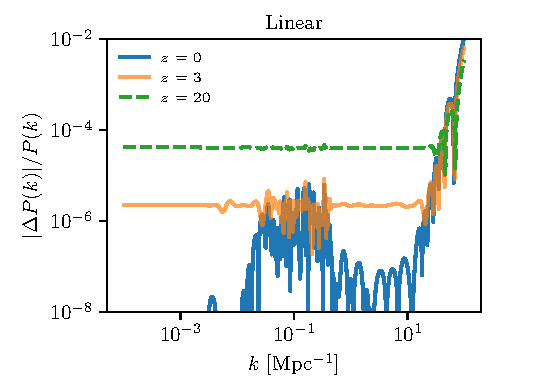
\includegraphics[width=0.49\textwidth]{splacc_power_lin}
  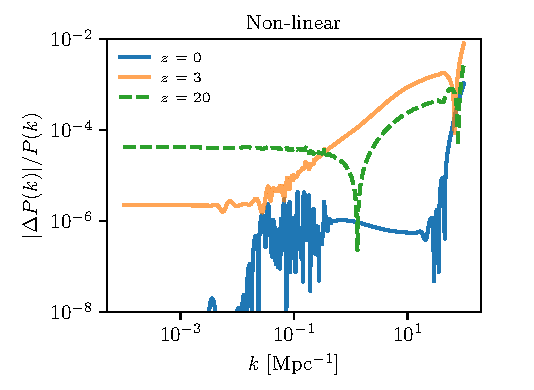
\includegraphics[width=0.49\textwidth]{splacc_power_nl}
\caption{The relative error compared to power spectra produced with high values of the power spectrum splines, $P_{fid}$, produced by splining the matter power spectrum up to {\tt K$\_$MAX$\_$SPLINE}$=50\,\text{Mpc}^{-1}$ and extrapolating beyond this value with a second order Taylor expansion the natural logarithm of the matter power spectrum. The left panel shows the relative errors for the linear matter power spectrum at $z=0$, $z=3$ and $z=20$. The right panel shows the results for the non-linear matter power spectrum at the same redshifts. The standard \ccl parameters adopted are those corresponding to the black dashed curve. For comparison, the impact of baryonic physics on the matter power spectrum is $\sim 10\%$ at $k=1\,\text{Mpc}^{-1}$ \citep{Schneider15}.}
\label{fig:NLextrapol}
\end{figure*}
%------------------------

\subsubsection{Extrapolation for the linear power spectrum}
\label{sec:Lextrapol}

With the implementation described in the previous section, the power spectrum splines are initialized up to {\tt K$\_$MAX$\_$SPLINE}. This is also true for the linear matter power spectrum, which is used within \ccl in particular to obtain $\sigma_8$ (see Eq. \ref{eq:sigR}). We have tested here how the procedure described in the previous section affects the convergence of the linear matter power spectrum. The result is shown in Figure \ref{fig:NLextrapol}. For some applications that use the linear power spectrum, the user might need to increase the value of {\tt K$\_$MAX$\_$SPLINE}.

As in the previous section, the power spectrum at small wavenumber is extrapolated using a power-law. This extrapolation is performed below a fiducial value of {\tt K\_MIN\_SPLINE} that coincides with the smallest wavenumber output by {\tt CLASS}, as in the case of the nonlinear power spectrum described above.

We have found that changing {\tt N$\_$A} to $200$, or changing the sampling of the wavenumber to $5000$ points, does not change the results presented in Figures \ref{fig:NLextrapol} in this section.

\subsubsection{Wishlist for the future}
\label{Pk_wishlist}
We plan to implement the following power spectrum methods in the future:
\begin{itemize}
 \item CAMB,
 \item other emulators,
 \item HOD.
\end{itemize}


\subsubsection{Normalization of the power spectrum}
\label{sec:PSnorm}

There are two alternative schemes for normalization of the matter power spectrum. The first one is to specify the value of $A_s$, the amplitude of the primordial power spectrum, which is passed directly to {\tt CLASS}. This option is available in the case of the linear/nonlinear matter power spectrum implementation. For these, as well as for BBKS and E\&H transfer functions, there is the additional option to set the normalization of the matter power spectrum by specifying $\sigma_8$, the RMS density contrast averaged over spheres of radius $8h^{-1}$Mpc. The computation of $\sigma_8$ is described in Section \ref{sec:hmf}.

In practice, there is only one argument that encodes the normalization. This is the argument ${\tt norm\_pk}$, which can be passed the power spectrum normalization parameterized by $\sigma_8$ or $A_\mathrm{s}$. As noted above, {\tt ccl$\_$parameters$\_$create} switches to $\sigma_8$ normalization if ${\tt norm\_pk} > 10^{-5}$, and to $A_{\mathrm s}$ normalization otherwise.

In the {\tt python} implementation, {\tt CCL} allows for either $\sigma_8$ or {\tt A\_s} to be passed as parameters.

\subsection{Angular power spectra}
\label{sec:cl}

In this section we will distinguish between {\sl observables} (quantities observed on the sky, such as number counts in a redshift bin, shear or CMB temperature fluctuations) and {\sl contributions} to the total observed fluctuations of these observables (such as the biased matter density term in number counts, redshift-space distortions, magnification, ISW, etc.).
The routines described in this subsection are implemented in {\tt ccl$\_$cls.cc}.

\subsubsection{Exact expressions}
The angular power spectrum between two observables $a$ and $b$ can be written as:
\begin{equation}
 C^{ab}_\ell=4\pi\int_0^\infty \frac{dk}{k}\,\mathcal{P}_\Phi(k)\Delta^a_\ell(k)\Delta^b_\ell(k),
\end{equation}
where $\mathcal{P}_\Phi(k)$ is the dimensionless power spectrum of the primordial curvature perturbations, and $\Delta^a$ and $\Delta^b$ are, using the terminology of CLASS, the transfer functions corresponding to these observables. Each transfer function will receive contributions from different terms. Currently \ccl supports two observables (also labelled ``tracers''), number counts and galaxy shape distortions, with the following contributions:
\paragraph{\bf Number counts.} The transfer function for number counts can be decomposed into three terms: $\Delta^{\rm NC}=\Delta^{\rm D}+\Delta^{\rm RSD}+\Delta^{\rm M}$, where
\begin{itemize}
  \item $\Delta^{\rm D}$ is the standard density term proportional to the matter density:
        \begin{equation}
          \Delta^{\rm D}_\ell(k)=\int dz\,p_z(z)\,b(z)\,T_\delta(k,z)\,j_\ell(k\chi(z)),
        \end{equation}
        where $T_\delta$ is the matter transfer function. Note that \ccl currently does not support non-linear or scale-dependent bias. Here, $p_z(z)$ is the normalized distribution of sources in redshift (selection function). Thus \ccl understands each individual redshift bin as a separate ``observable''.
  \item $\Delta^{\rm RSD}$ is the linear contribution from redshift-space distortions:
        \begin{equation}
          \Delta^{\rm RSD}_\ell(k)=\int dz\,p_z(z)\frac{(1+z) p_z(z)}{H(z)}T_\theta(k,z) j_\ell''(k\chi(z)),
        \end{equation}
        where $T_\theta(k,z)$ is the transfer function of $\theta$, the divergence of the comoving velocity field. $T_\theta(k,z)$ depends on the growth, which \ccl does not compute for massive neutrino cosmologies; therefore at this time an attempt to create a number count tracer in a cosmology with massive neutrinos will cause \ccl to raise an error. $C_\ell$ is instead computed assuming a linear-theory relation between the matter overdensity and peculiar velocity fields. While this should not be problematic for wide photometric redshift bins, users should exercise care when interpreting results for narrow window functions.
  \item $\Delta^{\rm M}$ is the contribution from magnification lensing:
        \begin{equation}
          \Delta_\ell^{\rm M}(k)=-\ell(\ell+1)\int \frac{dz}{H(z)} W^{\rm M}(z) T_{\phi+\psi}(k,z) j_\ell(k\chi(z)),
          \label{eq:deltaM}
        \end{equation}
        where $T_{\phi+\psi}$ is the transfer function for the Newtonian-gauge scalar metric perturbations, and $W^{\rm M}$ is the magnification window function:
        \begin{equation}
           W^{\rm M}(z)\equiv\int_z^\infty dz' p_z(z')\frac{2-5s(z')}{2}\frac{r(\chi(z')-\chi(z))}{r(\chi(z'))}.
        \end{equation}
        Here $s(z)$ is the magnification bias, given as the logarithmic derivative of the number of sources with magnitude limit, and $r(\chi)$ is the angular comoving distance (see Eq. \ref{eq:angdist}).

        Note that \ccl currently does not compute relativistic corrections to number counts \cite{2011PhRvD..84d3516C,2011PhRvD..84f3505B}. Although these should be included in the future, their contribution to the total fluctuation is largely subdominant (see \cite{GReffects} and the two references above), and therefore it is safe to work without them in most cases.
\end{itemize}

\paragraph{\bf Galaxy shape distortions.} The transfer function for shape distortions is currently decomposed into two terms: $\Delta^{\rm SH}=\Delta^{\rm WL}+\Delta^{\rm IA}$, where
\begin{itemize}
  \item $\Delta^{\rm L}$ is the standard lensing contribution:
        \begin{equation} \label{eq:transfer_lensing}
          \Delta_\ell^{\rm L}(k)=-\frac{1}{2}\sqrt{\frac{(\ell+2)!}{(\ell-2)!}}\int \frac{dz}{H(z)} W^{\rm L}(z) T_{\phi+\psi}(k,z) j_\ell(k\chi(z)),
        \end{equation}
        where $W^{\rm L}$ is the lensing kernel, given by
        \begin{equation}
          W^L(z)\equiv\int_z^\infty dz' p_z(z')\frac{r(\chi(z')-\chi(z))}{r(\chi(z'))}.
        \end{equation}
  \item $\Delta^{\rm IA}$ is the transfer function for intrinsic galaxy alignments. \ccl currently supports the so-called ``non-linear alignment model'', according to which the galaxy inertia tensor is proportional the local tidal tensor \cite{2004PhRvD..70f3526H,2007MNRAS.381.1197H}.
        \begin{equation}
          \Delta_\ell^{\rm IA}(k)=\sqrt{\frac{(\ell+2)!}{(\ell-2)!}}\int dz\,p_z(z)\,b_{\rm IA}(z)\,f_{\rm red}(z)\,T_\delta(k,z)\,\frac{j_\ell(k\chi(z))}{(k\chi(z))^2}.
        \end{equation}
\end{itemize}

It is worth noting that the equations above should be modified for non-flat cosmologies by replacing the spherical Bessel functions $j_\ell$ with their hyperspherical counterparts \cite{1994ApJ...432....7K}. Since the library currently only uses the Limber approximation (documented below), this is not currently an issue. It will be revisited in future versions of \ccl.

\paragraph{\bf CMB lensing.} The transfer function lensing convergence from a source at redshift $z_{\rm S}$ is given by:
\begin{equation} \label{eq:transfer_cmb_lensing}
  \Delta_\ell^{\rm C}(k)=-\frac{\ell(\ell+1)}{2}\int_0^{\chi_{\rm S}} d\chi\,\frac{r(\chi_{\rm S})-r(\chi)}{r(\chi)r(\chi_{\rm S})}T_{\phi+\psi}(k,\chi) j_\ell(k\chi),
\end{equation}
where $\chi_{\rm S}\equiv\chi(z_{\rm S})$.

\subsubsection{The Limber approximation}
As shown above, computing each transfer function involves a radial projection (i.e. an integral over redshift or $\chi$), and thus computing full power spectrum consists of a triple integral for each $\ell$. This can be computationally intensive, but can be significantly simplified in certain regimes by using the Limber approximation, given by:
\begin{equation}
 j_\ell(x)\simeq\sqrt{\frac{\pi}{2\ell+1}}\,\delta\left(\ell+\frac{1}{2}-x\right).
\end{equation}
Thus for each $k$ and $\ell$ we can define a radial distance $\chi_\ell\equiv(\ell+1/2)/k$, with corresponding redshift $z_\ell$. This approximation works best for wide radial kernels and high multipoles.

Substituting this in the expressions above, the simplified versions become:
\begin{equation}\label{eq:limber}
 C^{ab}_\ell=\frac{2}{2\ell+1}\int_0^\infty dk\,P_\delta\left(k,z_\ell\right)
 \tilde{\Delta}^a_\ell(k)\tilde{\Delta}^b_\ell(k).
\end{equation}
where
\begin{align}
 &\tilde{\Delta}_\ell^{\rm D}(k)=p_z(z_\ell)\,b(z_\ell)\,H(z_\ell)\\
 &\tilde{\Delta}_\ell^{\rm RSD}(k)=
 \frac{1+8\ell}{(2\ell+1)^2}\,p_z(z_\ell)\,f(z_\ell)\,H(z_\ell)-\\
 &\hspace{48pt}\frac{4}{2\ell+3}\sqrt{\frac{2\ell+1}{2\ell+3}}p_z(z_{\ell+1})\,f(z_{\ell+1})\,H(z_{\ell+1})\\
 &\tilde{\Delta}_\ell^{\rm M}(k)=3\Omega_{M,0}H_0^2\frac{\ell(\ell+1)}{k^2}\,
 \frac{(1+z_\ell)}{r(\chi_\ell)}W^{\rm M}(z_\ell)\\
 &\tilde{\Delta}_\ell^{\rm L}(k)=\frac{3}{2}\Omega_{M,0}H_0^2\sqrt{\frac{(\ell+2)!}{(\ell-2)}}\frac{1}{k^2}\,
 \frac{1+z_\ell}{r(\chi_\ell)}W^{\rm L}(z_\ell)\\
 &\tilde{\Delta}_\ell^{\rm IA}(k)=\sqrt{\frac{(\ell+2)!}{(\ell-2)!}}\frac{p_z(z_\ell)\,b_{\rm IA}(z_\ell)f_{\rm red}(z_\ell)H(z_\ell)}{(\ell+1/2)^2}\\
 &\tilde{\Delta}_\ell^{\rm C}(k)=\frac{3}{2}\Omega_{M,0}H_0^2\,\ell(\ell+1)\frac{1+z_\ell}{k^2}\,\frac{r(\chi_{\rm S})-r(\chi_\ell)}{r(\chi_\ell)r(\chi_{\rm S})}\,\Theta(\chi_\ell;0,\chi_{\rm S}).
\end{align}
Here ($\Theta(x;x_i,x_f)$) is a top-hat function (1 for $x\in[x_i,x_f]$ and 0 otherwise).

%----------------------------------------------------------------
%
%      Begin of the Angpow section currently under development
%
%----------------------------------------------------------------

\subsubsection{Beyond limber}

{\bf Native CCL computation.}

{\bf Note:} This capability has been deprecated in {\tt v1}, superseded by {\tt Angpow}, described below. But it is still available in previous versions of the library.

\ccl incorporates routines to compute the $C^{ab}_\ell$ angular power spectra as described above but without the Limber approximation. The algorithm performs first the integrals over $z$ for both tracers, and ends with the $k$ integral. This computation is much slower than using the Limber approximation, but it ends up with precise angular power spectra at low $\ell$, and correct cross-correlations between tracers (the Limber approximation fails at reproducing the interference terms $j_\ell(x)\times j_\ell(x')$).

Some parameters are needed to define this integral. First, to fasten the computation the $C^{ab}_\ell$ function is computed for a selection of $\ell$ values (linearly spaced at low-$\ell$ and logarithmicly spaced at high-$\ell$) and then the function is splined. Then the integration step of the redshift integrals must be specified in terms of a comoving distance. It is recommanded to start with a low value ($<3$\,Mpc) for a high precision integration, and then to release this parameter to achieve the user needs in terms of precision and rapidity. A logarithmic step in $k$ must also be provided: it does not correspond to the integration step but to a computation step before splining the transfer functions $\Delta^a_\ell(k)$. Last parameter, a minimum redshift can be given for the redshift integral bound so that the transfer functions are not computed near $z\approx 0$ where they can be numerically undefined.

The integration bounds in redshift are estimated automatically given the a redshift window so that the integration is preformed where the redshift window is relevant within a given precision (set by the \texttt{CCL\_FRAC\_RELEVANT} parameter). The integration bounds for the $k$ integrals are defined automatically given the $\ell$ multipole and the comoving distances at play.

It is worth noting that the user can define a threshold multipole $\ell$ from which the $C^{ab}_\ell$ computation switches to the Limber approximation which is faster and generally relevant at high $\ell$ values.

{\texttt{\bf Angpow}.}

The aim of the \texttt{Angpow} software \citep{2017arXiv170103592C} is to compute the angular power spectra  $C_{\ell}^{ab}$  without any Limber numerical approximation. \ccl has been linked to the \texttt{Angpow} code,  which is briefly described here.

The angular power spectrum for two shells $C_{\ell}^{ab}$ is computed in \texttt{Angpow} according to the following expression
\begin{equation}
  C_{\ell}^{ab} = \iint_0^\infty \mathrm{d} z \mathrm{d} z^\prime  p_{z_1}(z_1) p_{z_2}(z^\prime) \times \int_0^\infty \mathrm{d} k\ f_{\ell}(z, k) f_{\ell}(z^\prime, k).
  \label{eq-clz1z2-obs}
\end{equation}
The auxiliary function $f_\ell(z,k)$ can be defined without loss of generality as
\begin{equation}
f_\ell(z,k) \equiv  \sqrt{\frac{2}{\pi}}\  k \sqrt{P(k,z)}\ \widetilde{\Delta}_\ell(z,k)\label{eq-fell-func}
\end{equation}
with
\begin{itemize}
\item  $P(k,z)$ : the matter power spectrum at redshift $z$
\item $\widetilde{\Delta}_\ell(z,k)$: a function describing the physical processes such as matter density fluctuations, redshift-space distortions as described for instance in references \citet{2008cmb..book.....D,2009PhRvD..80h3514Y,2010PhRvD..82h3508Y, 2011PhRvD..84d3516C,2011PhRvD..84f3505B}. Currently, the \texttt{Angpow} version delivered with \ccl only can deal with galaxy clustering tracers (no lensing) and this without the magnification lensing term (equation \ref{eq:deltaM}). The incorporation of those transfer functions is left for future work, but in principle \texttt{Angpow} has already the capability to treat them. For now, for galaxy clustering tracers we defined $\widetilde{\Delta}_\ell(z,k)$ as
\begin{equation}
 \widetilde{\Delta}_\ell(z,k) \approx b j_\ell(k \chi(z)) - f(z) j_\ell^{\prime\prime}(k \chi(z))
\end{equation}
with $j_\ell(x)$ and $j_\ell^{\prime\prime}(x)$ the spherical Bessel function of order $\ell$ and its second derivative, and $f(a)$ the growth rate as defined subsection~\ref{sec:growth} (derivative of the growth function with respect to the scale factor $a$).
\end{itemize}

To proceed to a numerical evaluation of equation \ref{eq-clz1z2-obs}, \texttt{Angpow} first conducts  inside the rectangle $ [z_{1\mrm{min}},z_{1\mrm{max}}] \times [z_{2\mrm{min}},z_{2\mrm{max}}]$ given by the $p_z(z)$ selection functions a Cartesian product of one-dimensional (1D) quadrature
 defined by the set of sample nodes $z_i$ and weights $w_i$. In practice, the Clenshaw-Curtis quadrature is used.   The corresponding sampling points $(z_{1i},z_{2j})$ are weighted by the product  $w_i w_j$ using the 1D quadrature sample points and weights on both redshift regions with $i=0,\dots, N_{\mrm{z}_1}-1$ and $j=0,\dots,N_{\mrm{z}_2}-1$. Then, one gets the following approximation:
\begin{equation}
C_{\ell}^{ab} \approx  \sum_{i=0}^{N_{\mrm{z}_1}-1}\sum_{j=0}^{N_{\mrm{z}_2}-1} w_i w_j p_{z_1}(z_i)p_{z_2}(z_j) \widehat{P}_\ell(\chi_i,\chi_j)
\label{eq-cross-zquadra}
\end{equation}
with the notations $z_i = z_{1i}$, $z_j = z_{2j}$ and  $\chi_i = \chi(z_{1i})$, $\chi_j = \chi(z_{2j})$ and
\begin{equation}
\widehat{P}_\ell(z_i,z_j) =   \int_0^\infty dk\ f_\ell(z_i,k) f_\ell(z_j,k)
\label{eq-Pellzizj}
,\end{equation}
To conduct the computation of such integral of highly oscillating functions we use the 3C-algorithm described in details in reference \citep{2017arXiv170103592C}. In brief this algorithm proceeds the following way:
\begin{enumerate}
\item the total integration $k$ interval (eg. $[k_\mathrm{min}, k_\mathrm{max}]$) in equation (\ref{eq-Pellzizj}) is cut on several $k$-sub-intervals;
\item  on each sub-interval the functions $f_{i\, \ell}(k) = f_\ell(z_i,k) $ and $f_{j\, \ell}(k) = f_\ell(z_j,k)$ are projected onto Chebyshev series of order $2^N$;
\item the product of the two Chebyshev series is performed with a $2^{2N}$ Chebyshev series;
\item then, the integral on the sub-interval is computed thanks to the Clenshaw-Curtis quadrature.
\end{enumerate}
All the Chebyshev expansions and the Clenshaw-Curtis quadrature are performed via the DCT-I fast transform of FFTW.

Thanks to the 3C-algorithm, the \texttt{Angpow} is able to compute the $C_{\ell}^{ab}$ in a fast and accurate way. It was tested against \texttt{CLASS} and the native \ccl computation and can performed the computation an order of magnitude faster, which is more suitable for an extensive exploration of the cosmological parameter space ($\mathcal{O}(1s)$). Note that \texttt{Angpow} is written in C++ with OpenMP, to distribute the computation of a single $C_\ell$ on a single thread. The computation can also be switch by the user to the faster Limber approximation setting a threshold multipole $\ell$.


{\bf Precision tests.}

The code has been compared with \texttt{CLASS} and the native \ccl computation and all three softwares agrees perfectly if precision parameters are pushed to high levels.

A few parameters must be provided to set the precision of this computation. First the order of the Chebyshev polynomials is set to $2^{10}$ by default, and the number of $k$ sub-intervals to 200, and we checked this is enough for the current uses. Then the redshift quadrature stepping is set automatically given the redshift windows to recover the native \ccl computation boosted with high precision parameters: its precision is optimised so that the relative numerical error compared with the native method is two orders of magnitude below the relative cosmic variance $\sqrt{2/(2\ell+1)}$, from $\ell=2$ to $\ell=1000$. The $k_{\rm min}$ and $k_{\rm max}$ bounds are also automatically set given the current multipole $\ell$ and the comoving distance $\chi$ involved in the inner integral.




%----------------------------------------------------------------
%
%      End of the Angpow section currently under development
%
%----------------------------------------------------------------

\subsection{Correlation functions}
\label{sec:corr}


The following expressions relating the angular power spectra and correlation functions are valid in the flat-sky approximation\footnote{See the weak lensing review by \citet{Bartelmann01}, page 44 and \citet{Joachimi10}.}. In all cases, $f_K(\chi)$ is comoving angular diameter distance, which differs from the radial comoving distance $\chi$ only in the case of cosmologies with non-zero curvature. The routines described in this subsection are implemented in {\tt ccl$\_$correlation.c}.

{\bf Galaxy-galaxy.} The angular correlation function between two number-count tracers (labeled $a$ and $b$ here) is given by
\begin{equation}
  \xi^{ab}(\theta) = \int d\ell \frac{\ell}{2\pi} C^{ab}_\ell\, J_0(\ell\theta),
\label{eq:xiclu}
\end{equation}
where $C_{ab}$ is the angular power spectrum between both tracers.

{\bf Lensing-lensing.} The lensing correlation functions are \footnote{from Schneider 2002 and Bartelmann \& Schneider section 6.4.1}
\begin{eqnarray}
  \xi^{ab}_{+}(\theta)&=&\int_0^{\infty}d\ell\frac{\ell}{2\pi}J_0(\ell\theta)C^{ab}_\ell,\\
  \xi^{ab}_{-}(\theta)&=&\int_0^{\infty}d\ell\frac{\ell}{2\pi}J_4(\ell\theta)C^{ab}_\ell,
\label{eq:xipxim}
\end{eqnarray}
where the angular lensing convergence power spectrum $C^{ab}_\ell$ is given above (see Equations \ref{eq:transfer_lensing} and \ref{eq:limber}).

{\bf Galaxy-lensing.} The correlation between a number count tracer $a$ and a shear tracer $b$ is given by
\begin{equation}
  \xi^{ab}(\theta) = \int d\ell \frac{\ell}{2\pi} C^{ab}_\ell\, J_2(\ell\theta),
\end{equation}

Note that, in the above, ``Galaxy'' and ``Lensing'' can be replaced by any spin-0 and spin-2 fields on the sphere respectively (e.g. the CMB lensing convergence would play the same role as the galaxy overdensity field in all the formulas above).

{\bf 3d spatial correlation function.} In addition to the angular correlation functions, the 3-dimensional spatial correlation function $\xi(r)$ is also
calculated from the power spectrum $P(k)$ using
\begin{equation}
\xi(r) = \frac{1}{2 \pi^2} \int dk \; k^2 P(k) \frac{\sin(kr)}{kr}
\end{equation}


To evaluate the numerical integral in the correlation functions, we make use of the public code {\tt FFTlog}\footnote{\url{http://casa.colorado.edu/~ajsh/FFTLog/}}\citep{Hamilton2000,Talman2009}. In brief, {\tt FFTlog} works on functions periodic in log space, by writing the Hankel Transform as a convolution between Bessel functions and the function of interest (in this case either $C_\ell$ or $P(k)$). A version of this code is included in \ccl with minor modifications.


{\bf Redshift-space distortions.} In redshift space and under the linear approximation \citep{Kaiser1987} the correlation function $\xi(s,\mu)$ can be expanded in multipoles:
\begin{equation}
\xi(s,\mu) = \sum_{l\geq 0} \xi_l(s) L_l(\mu),
\end{equation}
where $s$ is the magnitude of the galaxy separation vector in redshift space $\bf s$, $\mu$ is the cosine of the separation angle between $\bf s$ and the line of sight, and $L_l(x)$ are the Legendre polynomials. The multipoles of the correlation function are given by
\begin{equation}
\xi_l(s) = \frac{i^l}{2 \pi^2} \int_0^{\infty} P_l(k) j_l(k s) k^2 dk,
\end{equation}
where $P_l(k)$ are multipoles of the power spectrum in redshift space $P(k,\mu_{\bf k})$ defined by
\begin{equation}
P(k,\mu_{\bf k}) = \sum_{l\geq 0} P_l(k) L_l(\mu_{\bf k}).
\end{equation}
In the linear approximation only the $l = 0,2,4$ multipoles are non-zero. They are related to the
real-space power spectrum $P(k)$ by
\begin{eqnarray}
&P_0(k) = \left(1+\frac{2}{3}\beta+\frac{1}{5}\beta^2\right)P(k),\\
&P_2(k) = \left(\frac{4}{3}\beta+\frac{4}{7}\beta^2\right)P(k),\\
&P_4(k) = \frac{8}{35}\beta^2 P(k),
\end{eqnarray}
where $\beta$ is the ratio of the growth rate $f$ and bias factor $b$, $\beta = f/b$.

\ccl implements the redshift space correlation function $\xi(s, \mu)$, it's average at constant $s$, $\xi(s)$,
the multiploes $\xi_l(s)$, and $\xi(\pi, \sigma)$, where $\pi$ is the galaxy pair separation
parallel to the line of sight and $\sigma$ is the separation perpendicular to the line of sight.
We use {\tt FFTlog} to calculate $\xi_l(s)$ from $P_l(k)$ in the implementation of $\xi(s,\mu)$.


In order to speed up the calculations, we provide the option to create a spline of the multipole functions $\xi_l(s)$ and store them in global splines for subsequent access. After calculating the redshift-space correlation functions for a given cosmology the splines should be freed using the provided function before calculating for a different cosmology.


%-----------------------------------------------------------
%
%   Correlation: beyond flat-sky (under development)
%
%-----------------------------------------------------------

\begin{comment}
\subsubsection{Beyond flat-sky}

We begin by writing the angular space observable, $X$, in terms of a decomposition in spherical harmonics,
\begin{align}\label{eq:X_harmonic}
  X(\Omega)=&\sum_{\ell m}\tilde X_{\ell m}Y_{\ell m}(\Omega)
\end{align}
where $\Omega$ refers to the angular coordinates on the sky.
The angular cross correlation function of two (scalar) tracers, $X$ and $Z$ of the large scale structure can be written in terms of their harmonic components, $\tilde X_{\ell m}$ and $\tilde Z_{\ell' m'}$ as
\begin{align}
  \langle XZ \rangle(\theta)=&\left\langle\sum_{\ell,m}\sum_{\ell', m'}\tilde X_{\ell m}\tilde Z_{\ell' m'}
  Y_{\ell m}(\Omega)
  Y_{\ell'm'}(\Omega+\theta)\right\rangle\\
  =&\sum_{\ell,m}C_{\ell}Y_{\ell m}(\Omega)
  Y_{\ell m}(\Omega+\theta)\\
  \langle XZ \rangle(\theta)=&\frac{1}{4\pi}\sum_{\ell}(2\ell+1)C_{\ell}P_{\ell}(\cos\theta)\label{eq:xi_pl0}
\end{align}
where we have used the identities
\begin{align}
  \langle\tilde X_{\ell m}\tilde Z_{\ell' m'}\rangle=&C_{\ell}\delta_D(m,m')\delta_D(\ell,\ell'),\\
  \sum_{m=-\ell}^{m=\ell}Y_{\ell m}(\Omega)Y_{\ell m}(\Omega+\theta)=&\frac{2\ell+1}{4\pi}\label{eq:Ylm_Pl}.
\end{align}

For the case of shear, since it is a spin-2 object, eq.\ref{eq:X_harmonic} is written in terms of spin harmonics
\citep[see for ex.][]{Castro2005,Kilbinger2017}. The rest of the analysis proceeds similarly, using the relation for spin
harmonics, analogous to eq.~\ref{eq:Ylm_Pl} \citep[see for ex. ][]{Hu1997}.

The expressions for $\xi_+$ (which is the same as in Eq.~\ref{eq:xi_pl0}) and for $\xi_-$ are given by
\begin{align}
  %\langle g\gamma_T\rangle(\theta)&=\frac{1}{4\pi}\sum_{\ell}\frac{(2\ell+1)}{\ell(\ell+1)}C_{\ell}^{g\kappa}
  %P_{\ell}^2(\cos\theta)\label{eq:xi_g_gamma}\\
  \xi_+(\theta)&=\frac{1}{4\pi}\sum_{\ell}{(2\ell+1)}C_{\ell}^{\kappa\kappa}
  P_{\ell}(\cos\theta)\label{eq:xi_p}\\
  \xi_-(\theta)&=\frac{1}{4\pi}\sum_{\ell}\frac{(\ell-4)!}{(\ell+4)!}\ell^4{(2\ell+1)}C_{\ell}^{\kappa\kappa}
  P_{\ell}^4(\cos\theta)\label{eq:xi_m}
\end{align}
\todo{Simply took the relation between $P_\ell^m$ and $J_m(\ell \theta)$ to get this expression from the Hankel transform for $\xi_-$. It may not be very accurate at large scale (low $\ell$) as is evident from $g\gamma_T$ expression. To be revisited.}

The {\tt ccl\_tracer\_corr\_legendre} routine computes these transform to convert angular power spectra, $C_\ell$, into correlation functions. We use the associated Legendre function implementation from the {\tt GSL} library. {\tt ccl\_tracer\_corr\_legendre} routine evaluations can be very slow, especially for polynomials $P_\ell^m$ with $m>0$. Note that $P_\ell^m$ evaluations need to be done only once and can then be saved as long as $\ell$ and $\theta$ values do not change. However, \ccl has not yet implemented this feature.

\paragraph{Hankel Transform}
Notice that in the flat-sky limit, the expressions in Eqs.~\ref{eq:xi_p}--\ref{eq:xi_m} can be written as Hankel transforms using the relation between $P_{\ell}^m$ and bessel functions $J_m$
\begin{align}
  P_{\ell}^m(\cos\theta)=(-1)^m\frac{(\ell+m)!}{(\ell-m)!}\ell^{-m}J_m(\ell\theta)
\end{align}
which yields final expressions that coincide with Eq. \ref{eq:xipxim}.

\end{comment}


%-----------------------------------------------------------
%
%   End of Correlation: beyond flat-sky (under development)
%
%-----------------------------------------------------------


\subsection{Halo mass \& halo bias functions}
\label{sec:hmf}

The routines described in this subsection are implemented in {\tt ccl$\_$massfunc.c}.

The halo mass function is implemented using several different definitions from the literature: \citet{Tinker2008}, \citet{Tinker2010}, \citet{Angulo2012}, and \citet{Watson2013}. All four models are tuned to simulation data and tested against observational results. In addition, each of these fits has been implemented using the common halo definition of $\Delta = 200$, where a halo is defined with:
\begin{equation}
\bar{\rho}(r_{\Delta}) = \Delta \times \rho_{\mathrm{m}},
\end{equation}
where a halo with size $r_{\Delta}$ has an average density $\bar{\rho}$ equal to the overdensity parameter $\Delta$ times the mean background density of the universe, $\rho_{\mathrm{m}}$. Note that another common definition utilizes the critical density of the universe, $\rho_{\mathrm{c}}$; currently \ccl requires that an external conversion by the end user between values of $\Delta$ with respect to the critical density to values of $\Delta$ as defined with respect to the mean density. In the future we plan to allow for self-consistent handling of critical density based definitions, though it is not implemented as of this build.

In addition to the usage of the most common definition, we have implemented an extension for two of the models. The Tinker 2010 model allows for a value of $\Delta$ to be given between the values of 200 and 3200 and interpolates the fitting parameters within this range in a space of $\log \Delta$ using splines. We also have implemented interpolation in the same range of Tinker 2008 $\Delta$ values. For both Tinker 2008 and Tinker 2010 models we have utilized spline interpolation through {\tt GSL} routines in order to guarantee a match to specified fitting parameters at exact values of $\Delta$. This fitting has slight deviation from the fit as expressed in Tinker 2010.

The halo mass function models implemented in CCL are tuned to simulations without massive neutrinos, therefore are not valid in cosmologies with massive neutrinos. Attempts to calculate the halo mass function, halo bias, or other related quantities within cosmologies with massive neutrinos will cause \ccl to raise an error and quit.


With the exception of the Tinker 2010 model, we attempt to keep a common form to the multiplicity function whenever possible for ease of extension:
\begin{equation}
f(\sigma)=A\Big[\Big(\frac{\sigma}{b}\Big)^{-a}+1\Big]e^{-c/{\sigma}^2},
\end{equation}
where $A$, $a$, $b$, and $c$ are fitting parameters that have additional redshift scaling and $\sigma$ is the RMS variance of the density field smoothed on some scale $M$ at some scale factor $a$. This basic form is modified for the \citet{Angulo2012} formulation. The resulting form is
\begin{equation}
f(\sigma)=A\Big[\Big(\frac{b}{\sigma}+1\Big)^{-a}\Big]e^{-c/{\sigma}^2},
\end{equation}
where the only change is in the formulation of the second term. Note that the fitting parameters in the \citet{Angulo2012} formulation do not contain any redshift dependence and the use of it is primarily for testing and benchmark purposes.

Each call to the halo mass function requires an assumed model (defined within the {\tt ccl$\_$configuration} structure contained in {\tt ccl$\_$cosmology}), in addition to a value of the halo mass and scale factor for which to evaluate the halo mass function. The currently implemented models can be called with the tags {\tt config.mass$\_$function$\_$method = ccl$\_$tinker}, {\tt ccl$\_$tinker10}, {\tt ccl$\_$angulo}, or {\tt ccl$\_$watson}. It returns the number density of halos in logarithmic mass bins, in the form $dn/d\log_{10}{M}$, where $n$ is the number density of halos of a given mass and $M$ is the input halo mass.

The halo mass $M$ is related to $\sigma$ by first computing the radius $R$ that would enclose a mass $M$ in a homogeneous Universe at $z=0$:
\begin{equation}
  M=\frac{H_0^2}{2G}R^3\,\rightarrow \frac{M}{M_\odot}=1.162\times10^{12}\Omega_Mh^2\,\left(\frac{R}{1\,{\rm Mpc}}\right)^3.
\end{equation}
The rms density contrast in spheres of radius $R$ can then be computed as
\begin{equation}
  \sigma_R^2 = \frac{1}{2\pi^2}\int dk\,k^2\,P_k\,\tilde{W}_R^2(k)
  \label{eq:sigR}
\end{equation}
where $P_k$ is the matter power spectrum and $\tilde{W}(kR)$ is the Fourier transform of a spherical top hat window function,
\begin{equation}
\tilde{W}_R(k) = \frac{3}{(kR)^3}[\sin(kR)-kR\cos(kR)]
\end{equation}
%
This function is directly implemented in \ccl as well as a specific $\sigma_8$ function.

The \citet{Tinker2010} model parameterizes both the halo mass function and the halo bias in terms of the peak height, $\nu = \delta_c / \sigma(M)$, where $\delta_c$ is the critical density for collapse and is chosen to be $1.686$ for this particular parameterization. We can then parameterize the halo function and halo bias as
\begin{equation}
  b(\nu) = 1 - A\frac{\nu^a}{\nu^a + {\delta_c}^a} + B\nu^b+C\nu^c,
  f(\nu) = \alpha[1+(\beta\nu)^{-2\phi}]\nu^{2\eta}e(-\gamma\nu^2/2).
  \label{eq:halo_bias_and_mass_function}
\end{equation}
The currently implemented model in \ccl allows for an arbitrary overdensity $\Delta$ to be chosen, using the fitting functions provided in \citet{Tinker2010}. Other halo model definitions are not included in the halo bias calculation, though this remains an area of active work to improve upon.


% Written by Alexander Mead
\subsection{Halo model}
\label{sec:halo_model}

The routines described in this subsection are implemented in {\tt ccl$\_$halomod.c}.

In this section we review a basic halo-model computation \citep{Seljak2000,Peacock2000,Cooray2002} of the cross-correlation between any two cosmological fields and only requires knowledge of the halo profiles of the field in question. For example, in the case of the matter-density auto spectrum we need only know the halo density profiles. For the galaxy spectrum we require knowledge of the number of, and distribution of, galaxies as a function of halo mass. In this simple form the halo model is approximate and makes the assumption that haloes are \emph{linearly} biased with respect to the \emph{linear} matter field and also assumes that haloes are spherical with properties that are determined solely by the halo mass. It is possible to go beyond these simplified assumptions, and we direct the interested reader to \cite{Cooray2002,Smith2007,Giocoli2010,Smith2011}.

The eventual aim for CCL is to have a halo model that can calculate the auto- and cross-spectra for any cosmological field combinations with parameters that can be taken either from numerical simulations or observational data. Currently we have only implemented the case of the matter-density auto spectrum, but we keep the notation as general as possible in the following:

Consider two 3D cosmological fields $\rho_i$ and $\rho_j$, the cross power spectrum at a given redshift can be written as a sum of a two- and a one-halo term given by
\begin{equation}
P_{2\mathrm{H},ij}(k)=P_{\mathrm{lin}}(k)
\prod_{n=i,j}\left[\int_0^\infty b(M)\frac{\mathrm{d}n}{\mathrm{d}M}W_n(M,k)\;\mathrm{d}M\right]\ ,
\label{eq:two_halo}
\end{equation}
\begin{equation}
P_{1\mathrm{H},ij}(k)=\int_0^\infty \frac{\mathrm{d}n}{\mathrm{d}M}W_i(M,k)W_j(M,k)\;\mathrm{d}M\ ,
\label{eq:one_halo}
\end{equation}
where $M$ is the halo mass, $\mathrm{d}n/\mathrm{d}M$ is the halo mass function defined as the first of equations~(\ref{eq:halo_bias_and_mass_function}) and $b(M)$ is the linear halo bias with respect to the linear matter density field, defined as the large-scale limit of the second of equations~(\ref{eq:halo_bias_and_mass_function}).

Equations~(\ref{eq:two_halo}) and (\ref{eq:one_halo}) contain the (spherical) Fourier transform of the halo profile, or halo `window function':
\begin{equation}
W_i(M,k)=\int_0^\infty4\pi r^2\frac{\sin(kr)}{kr}\rho_{\mathrm{H},i}(M,r)\;\mathrm{d}r\ ,
\label{eq:window_function}
\end{equation}
where $\rho_{\mathrm{H},i}(M,r)$ is the radial profile for the field $i$ in a host halo of mass $M$. For example, if one is interested in matter fields then this would be the halo density profile, if one were interested in galaxies then this would be the number density and distribution of galaxies around a halo of mass $M$.

Note that the halo mass function and bias \emph{must} satisfy the following properties for the total power spectrum to have the correct large-scale limit\footnote{Note that achieving these correct limits for some fields is difficult numerically because of the large amount of mass contained in low mass haloes according to most popular mass functions. Special care must be taken with the two-halo integral in the case of matter power spectra.}:
\begin{equation}
\frac{1}{\bar\rho_\mathrm{m}}\int_0^\infty M\frac{\mathrm{d}n}{\mathrm{d}M}\;\mathrm{d}M=1\ ,
\label{eq:mf_normalisation}
\end{equation}
\begin{equation}
\frac{1}{\bar\rho_\mathrm{m}}\int_0^\infty Mb(M)\frac{\mathrm{d}n}{\mathrm{d}M}\;\mathrm{d}M=1\ .
\label{eq:bias_normalisation}
\end{equation}
If one uses a mass function and bias pair that are related via the peak-background split formalism \citep{Mo1996,Sheth2001}, these conditions are automatically satisfied. In words these equations enforce that all matter is associated to a halo and that matter is on average unbiased with respect to itself. In the convention used in CCL the units of $P(k)$ will be exactly the units of $\rho_i\rho_j / \mathrm{Mpc}^3$. The units of the $W_i$ are those of $\rho_i$ multiplied by volume.

For the matter power spectrum we use the halo profiles of \citeauthor*{Navarro1997} (NFW; \citeyear{Navarro1997}):
\begin{equation}
\rho_\mathrm{H}(M,r)\propto\frac{1}{r/r_\mathrm{s}(1+r/r_\mathrm{s})^2}\ ,
\label{eq:NFW_profile}
\end{equation}
which is written in terms of a scale radius $r_\mathrm{s}$. The constant of proportionality fixed by the condition that the halo has total mass $M$ when the boundary is set at the virial radius $r_\mathrm{v}$, which is set such that the halo has a fixed density $\Delta_\mathrm{v}$ with respect to the mean
\begin{equation}
M=4\pi r_\mathrm{v}^3\Delta_\mathrm{v}\bar\rho\ .
\label{eq:virial_radius}
\end{equation}
Finally, the scale radius is usually expressed in terms of the mass-dependent halo concentration parameter $c(M)=r_\mathrm{v}/r_\mathrm{s}$. We use the simple mass-concentration relation from \cite{Bullock2001}
\begin{equation}
c(M)=9\left(\frac{M}{M_*}\right)^{-0.13}\ ,
\end{equation}
where $\delta_\mathrm{c}/\sigma(M_*)=1$.
Note that, in order to be consistent, one should use a value of $\Delta_\mathrm{v}$ and $c(M)$ that is consistent with the halo definition used for the halo mass function and bias.


\section{Tests and validation}
\label{sec:tests}

Our goal is for outputs of \ccl to be validated against independent benchmark codes. This process is documented in the \ccl paper that can be found in the {\tt doc/ccl\_paper} folder.

For each \ccl prediction, at least one independent code was used to produce the same result. Predictions were compared and the resulting numerical accuracy, documented in the paper. (See Table 2 for a summary of these results.) Potential differences in the implementation of the relevant algorithms were discussed there as well. For specific cases, such as the matter power spectrum provided by the Cosmic Emulator, angular power spectra and projected correlation functions, we established target accuracies for \ccl to achieve, though a more detailed forecasting exercise should be pursued in the future to establish whether results are compatible with the expected requirements of LSST DESC cosmological analyses in the next decade.

All benchmark codes are either made public within the \ccl repository or made available online and described in the \ccl wiki\footnote{\url{https://github.com/LSSTDESC/CCL/wiki}}.

\ccl has a suite of test routines which, upon compilation, compare its outputs to the benchmarks from code comparison. These are run from the \ccl root directory with the command {\tt ./build/check\_ccl}.

\section{Examples for C implementation}
\label{sec:example}

Examples of how to run \ccl are provided in the {\tt examples} sub-directory of the library. The first resource for a new user should be the {\tt ccl$\_$sample$\_$run.c} file. This starts by setting up the \ccl default configuration. Then, it creates the {\tt cosmo} structure, which contains distances and power spectra splines, for example. There are example calls for routines that output comoving radial distances, the scale factor, the growth factor and $\sigma_8$. Toy models are created for the redshift distributions of galaxies in the clustering and lensing samples, and for the bias of the clustering sample ($b(z)=1+z$). These are used for constructing the ``tracer'' structures via {\tt CCL$\_$Cltracer}, which can then be called to obtain the angular power spectra for clustering, cosmic shear and CMB lensing. All functions of redshift associated to each tracer can be retrieved at any arbitrary point using the same interpolation scheme used by \ccl internally.


\section{Python example}
\label{sec:python:example}

A Python wrapper for \ccl is provided through a module called {\tt pyccl}. The whole \ccl interface can be accessed through regular Python functions and classes, with all of the computation happening in the background through the C code. The functions all support {\tt numpy} arrays as inputs and outputs, with any loops being performed in the C code for speed.

The Python module has essentially the same functions as the C library, just presented in a more standard Python-like way. You can inspect the available functions and their arguments by using the built-in Python {\tt help()} function, as with any Python module.

Below is a simple example Python script that creates a new {\tt Cosmology} object, and then uses it to calculate the $C_\ell$'s for a simple lensing cross-correlation. It should take a few seconds on a typical laptop.
\begin{verbatim}
import pyccl as ccl
import numpy as np

# Create new Cosmology object with a given set of parameters. This keeps track
# of previously-computed cosmological functions
cosmo = ccl.Cosmology(Omega_c=0.27, Omega_b=0.045, h=0.67, A_s=2e-9, n_s=0.96)

# Define a simple binned galaxy number density curve as a function of redshift
z_n = np.linspace(0., 1., 200)
n = np.ones(z_n.shape)

# Create objects to represent tracers of the weak lensing signal with this
# number density (with has_intrinsic_alignment=False)
lens1 = ccl.WeakLensingTracer(cosmo, dndz=(z_n, n))
lens2 = ccl.WeakLensingTracer(cosmo, dndz=(z_n, n))

# Calculate the angular cross-spectrum of the two tracers as a function of ell
ell = np.arange(2, 10)
cls = ccl.angular_cl(cosmo, lens1, lens2, ell)
print cls
\end{verbatim}

Further examples are collected in several Jupyter notebooks available in the {\tt examples/} directory. These are:
\begin{verbatim}
Correlation.ipynb,

Distance Calculations Example.ipynb,

HMFexample.ipynb,

Lensing angular power spectrum.ipynb,

MCMC Likelihood Analysis.ipynb,

Photo-z example.ipynb,

Correlation_3d.ipynb,

Power spectrum example.ipynb
\end{verbatim}

Note that the likelihood analysis in the last notebook is not intended to be realistic, but it gives an operational example of how {\tt CCL} can be integrated into such an analysis. In particular, the notebook only considers cosmic shear over one wide redshift bin and the covariance matrix adopted solely includes a contribution from cosmic variance. The ``data vector'' is simply a simulated using {\tt CCL} theoretical predictions. For speed, theoretical predictions use the BBKS power spectrum implementation.


\section{Technical notes on how the Python wrapper is implemented}
\label{sec:python:technical}

The Python wrapper is built using the {\tt swig} tool, which automatically scans the \ccl C headers and builds a matching interface in Python. The default autogenerated {\tt swig} interface can be accessed through the {\tt pyccl.lib} module if necessary. A more user-friendly wrapper has been written on top of this to provide more structure to the module, allow {\tt numpy} vectorization, and provide more natural Python objects to use (instead of opaque {\tt swig}-generated objects).

The key parts of the wrapper are as follows:
\paragraph{{\tt setup.py}} This instructs {\tt swig} and other build tools on how to find the right source files and set compile-time variables correctly. Most of this information is provided by header files and SWIG interface files that are included through the {\tt pyccl/ccl.i} interface file.

Note that certain compiler flags, like {\tt -fopenmp}, are also set in {\tt setup.py}. If you are not using {\tt gcc}, you may need to modify these flags (see the {\tt extra$\_$compile$\_$args} argument of the {\tt setup()} function).

\paragraph{Interface ({\tt .i}) files} These are kept in the {\tt pyccl/} directory, and tell {\tt swig} which functions to extract from the C headers. There are also commands in these files to generate basic function argument documentation, and remove the {\tt ccl$\_$} prefix from function names.

The interface files also contain code that tells {\tt swig} how to convert C array arguments to {\tt numpy} arrays. For certain functions, this code may also contain a simple loop to effectively vectorize the function.

The main interface file is {\tt pyccl/ccl.i}, which imports all of the other interface files. Most of the \ccl source files (e.g. {\tt core.c}) have their own interface file too. For other files, mostly containing support/utility functions, {\tt swig} only needs the C header ({\tt .h}) file to be specified in the main {\tt ccl.i} file, however. (The C source file must also be added to the list in {\tt setup.py} for it to be compiled successfully.)

\paragraph{Python module files} The structure of the Python module, as seen by the user, is organized through the {\tt pyccl/$\_$$\_$init$\_$$\_$.py} file, which imports only the parts of the {\tt swig} wrapper that are useful to the user. The complete autogenerated {\tt swig} interface can be accessed through the {\tt pyccl.lib} sub-module if necessary.

Individual sub-modules from \ccl are wrapped in their own Python scripts (e.g. {\tt power.py}), which typically provide a nicer ``Pythonic'' interface to the underlying \ccl functions and objects. This includes automatically choosing whether to use the vectorized C function or not, as well as some conversions from Python objects to the autogenerated {\tt swig} objects. Most of the core Python objects, like {\tt Cosmology}, are defined in {\tt core.py}. These objects also do some basic memory management, like calling the corresponding {\tt ccl$\_$free$\_$*} C function when the Python object is destroyed.

\paragraph{Auto-generated wrapper files} The {\tt swig} command is triggered when you run {\tt setup.py}, and automatically generates a number of C and Python wrapper files in the {\tt pyccl/} directory. These typically have names like {\tt ccl$\_$*.c} and {\tt ccl$\_$*.py}, and should not be edited directly, as {\tt swig} will overwrite them when it next runs.

\paragraph{{\tt pyccl/pyutils.py}} This file contains several generic helper functions for passing {\tt numpy} arrays in and out of Python functions in a convenient way, and for performing error checking and some type conversions.

The build process will also create a {\tt pyccl/ccllib.py} file, which is the raw autogenerated Python interface, and {\tt $\_$ccllib.so}, which is a C library containing all of the C functions and their Python bindings. A {\tt build/} directory and {\tt pyccl.egg-info/} directory will also be created in the same directory as {\tt setup.py} when you compile {\tt pyccl}. These (plus the {\tt pyccl/$\_$ccllib.so} file) should be removed if you want to do a clean recompilation. Running {\tt python setup.py clean --all} will remove some, but not all, of the generated files.


\section{Future functionality to be included}
\label{sec:future}

In the future, we hope that \ccl will include other functionalities. Functionalities which are currently under development:
\begin{itemize}
\item further CMB observable predictions (beyond CMB lensing)\footnote{\url{https://github.com/LSSTDESC/CCL/issues/428}},
\item support for non-linear biasing models\footnote{\url{https://github.com/LSSTDESC/CCL/pull/444}}\citep[e.g.][]{FASTPT},
\item halo density profiles\footnote{\url{https://github.com/LSSTDESC/CCL/issues/407}},
\item velocity correlation function\footnote{\url{https://github.com/LSSTDESC/CCL/issues/429}},
\item mass function emulators\footnote{\url{https://github.com/LSSTDESC/CCL/issues/235}},
\item and more power spectrum methods (see \ref{Pk_wishlist}).
\end{itemize}

\section{Feedback}
\label{sec:feedback}

If you would like to provide feedback on \ccl or contact the administrators, please do so through the \ccl github repository located at \url{https://github.com/LSSTDESC/CCL}. We welcome users opening github issues.

\section{Citing \& using \ccl}
\label{sec:cite}

This software is a publicly released LSST DESC product which was developed within the LSST DESC using LSST DESC resources. DESC users should use it in accordance with the LSST DESC publication policy\footnote{\url{http://lsstdesc.org/Collaborators}}. External users are welcome to use the code outside DESC in accordance with the licensing information below.

This code has been released by DESC, although it is still under active development. It is accompanied by a journal paper that describes the development and validation of the library, which you can find the in the {\tt doc/ccl\_paper} folder. You are welcome to re-use the code, which is open source and available under terms consistent with our LICENSE\footnote{\url{https://github.com/LSSTDESC/CCL/blob/master/LICENSE}}, which is a BSD 3-Clause\footnote{\url{https://opensource.org/licenses/BSD-3-Clause}} license.

For free use of the {\tt CLASS} library, the {\tt CLASS} developers require that the {\tt CLASS} paper be cited: {\it  CLASS II: Approximation schemes}, D. Blas, J. Lesgourgues, T. Tram, arXiv:1104.2933, JCAP 1107 (2011) 034. The {\tt CLASS} repository can be found in \url{http://class-code.net}.

\section{License}
\label{sec:license}

Copyright \textcopyright 2016-2018, the LSST DESC \ccl contributors (https://github.com/LSSTDESC/CCL/graphs/contributors). The repository can be found at \url{https://github.com/LSSTDESC/CCL}. All rights reserved.

Redistribution and use in source and binary forms, with or without
modification, are permitted provided that the following conditions are met:

\begin{itemize}
\item Redistributions of source code must retain the above copyright notice, this
  list of conditions and the following disclaimer.
\item Redistributions in binary form must reproduce the above copyright notice,
  this list of conditions and the following disclaimer in the documentation
  and/or other materials provided with the distribution.
\item Neither the name of \ccl (\url{https://github.com/LSSTDESC/CCL}) nor the names of its
  contributors may be used to endorse or promote products derived from
  this software without specific prior written permission.
\end{itemize}

THIS SOFTWARE IS PROVIDED BY THE COPYRIGHT HOLDERS AND CONTRIBUTORS ``AS IS''
AND ANY EXPRESS OR IMPLIED WARRANTIES, INCLUDING, BUT NOT LIMITED TO, THE
IMPLIED WARRANTIES OF MERCHANTABILITY AND FITNESS FOR A PARTICULAR PURPOSE ARE
DISCLAIMED. IN NO EVENT SHALL THE COPYRIGHT HOLDER OR CONTRIBUTORS BE LIABLE
FOR ANY DIRECT, INDIRECT, INCIDENTAL, SPECIAL, EXEMPLARY, OR CONSEQUENTIAL
DAMAGES (INCLUDING, BUT NOT LIMITED TO, PROCUREMENT OF SUBSTITUTE GOODS OR
SERVICES; LOSS OF USE, DATA, OR PROFITS; OR BUSINESS INTERRUPTION) HOWEVER
CAUSED AND ON ANY THEORY OF LIABILITY, WHETHER IN CONTRACT, STRICT LIABILITY,
OR TORT (INCLUDING NEGLIGENCE OR OTHERWISE) ARISING IN ANY WAY OUT OF THE USE
OF THIS SOFTWARE, EVEN IF ADVISED OF THE POSSIBILITY OF SUCH DAMAGE.

% 
We would like to thank the organisers of the the DESC collaboration meetings at:
Oxford (July 2016), SLAC (March 2016), and ANL (2015), 
and the LSST-DESC Hack Week organisers (CMU, November 2016), where this work 
was partly developed. We would also like to acknowledge the
contribution of the participants of the TJP Code Comparison Project, some of whom
are among the CCL contributors, for providing the benchmarks for 
testing CCL. Finally, we are grateful for the feedback received from
other working groups of DESC, including Strong Lensing, Supernovae
and Photometric Redshifts.
% 


Author contributions are listed below. \\
Husni Almoubayyed: wrote an mcmc jupyter notebook example, reviewed code/contributed to issues. \\
David Alonso: Co-led project; developed structure for angular power spectra; implemented autotools; integrated into LSS pipeline; contributed to: background, power spectrum, mass function, documentation and benchmarks; reviewed code \\
M.~R.~Becker: Core code and algorithmss \\
Jonathan Blazek: Planning capabilities and structure; documentation and testing. \\
Philip Bull: Implemented the Python wrapper and wrote documentation for it; general bug fixes, maintenance, and code review; enhanced the installer and error handling system. \\
Jean-\'Eric Campagne: Angpow builder and contributed to the interface with CCL. \\
N. Elisa Chisari: Co-led project, coordinated hack projects \& communication, contributed to: correlation function \& power spectrum implementation, documentation, and comparisons with benchmarks. \\
Alex Drlica-Wagner: Helped with document preparation. \\
Zilong Du: Implemented the 3d correlation function, redshift-space correlation functions, and corresponding benchmarks. \\
Tim Eifler: Reviewed/tested code. \\
John Ellison: Implemented the 3d correlation function, redshift-space correlation functions, and corresponding benchmarks; wrote documentation. \\
Cristhian Garcia Quintero: Produced benchmarks for correlation functions in modified gravity. \\
Ren\'ee Hlozek: Contributed initial code for error handling structures, reviewed other code edits. \\
Mustapha Ishak: Contributed to planning of code capabilities and structure; reviewed code; identified and fixed bugs. \\
Shahab Joudaki: Created physical density function and documentation. \\
Matthew Kirby: Performed comparison of physical constants. \\
David Kirkby: Writing, testing and reviewing code. Asking questions. \\
Elisabeth Krause: Initiated and co-led project; developed CLASS interface and error handling; contributed to other code; reviewed pull requests. \\
Francois Lanusse: Worked on install procedure \\
C. Danielle Leonard: Wrote and tested code for LSST specifications, user-defined photo-z interface, and support of massive neutrinos; reviewed other code; wrote text for this note. \\
Christiane S. Lorenz: Contributed to accurate high-redshift cosmological background quantities and benchmarked background splines. \\
Phil Marshall: Helped with document preparation. \\
Thomas McClintock: Wrote Python documentation. \\
Sean McLaughlin: Wrote doxygen documentation and fixed bugs/added functionality to distances. \\
Alexander Mead: Wrote halo model code \\
J\'er\'emy Neveu: Contributed to Angpow and built the interface with CCL. \\
St\'ephane Plaszczynski: Contributed to Angpow and contributed to the interface with CCL. \\
Javier Sanchez: Modified setup.py to allow pip installation and uninstall. \\
Sukhdeep Singh: Contributed to the correlation functions code. \\
An\v{z}e Slosar: Wrote and reviewed code. \\
Tilman Tr\"oster: Wrote code for user-changable precision parameters, added distance and growth factor tests, found and fixed bugs. \\
Antonio Villarreal: Contributed to initial benchmarking, halo mass function code, and general code and issues review. \\
Michal Vrastil: Wrote documentation and example code, reviewed code. \\
Kuan Wang: Wrote halo profiles code. \\
Joe Zuntz: Wrote initial infrastructure, C testing setup, and reviewed code. \\


%{\it Facilities:} \facility{LSST}

\bibliography{main}

\end{document}
%
